\documentclass[manuscript, nonacm]{acmart}

\usepackage{xcolor}
\usepackage{tikz}
\usetikzlibrary{shapes.geometric, arrows.meta, positioning, decorations.pathreplacing}
\usepackage{pgfplots}
\pgfplotsset{compat=1.18}
% figure palette, kept muted so diagrams do not dominate the page
\definecolor{figblue}{RGB}{48,84,150}
\definecolor{figgreen}{RGB}{51,140,83}
\definecolor{figorange}{RGB}{176,111,38}
\definecolor{figred}{RGB}{170,60,60}
\definecolor{figgrid}{RGB}{218,218,218}

\pgfplotsset{
    every axis/.append style={
        tick label style={font=\small},
        label style={font=\small},
        title style={font=\small},
        axis line style={gray!65},
        tick style={gray!65},
        grid style={figgrid},
    },
}
\usepackage{listings}
\usepackage{booktabs}
\usepackage{array}
\usepackage{tcolorbox}
\usepackage{url}
\usepackage{float}
\usepackage{placeins}
\usepackage{needspace}

% code listing style
\definecolor{kwblue}{RGB}{0,0,200}
\definecolor{listbg}{RGB}{245,245,250}

\lstdefinelanguage{Sollya}{
    morekeywords={prec,display,hexadecimal,decimal,rationalmode,off,
    guessdegree,remez,fpminimax,dirtyinfnorm,infnorm,supnorm,
    horner,canonical,round,evaluate,sup,inf,log2,log,exp,sin,cos,
    print,for,from,to,do,if,then,else,version,D,RN,relative,absolute},
    sensitive=true,
    morecomment=[l]{//},
    morestring=[b]",
}

% fullflexible columns keep hex float literals such as 0x1.5555p-3 intact
% instead of letting fixed-column alignment scatter them
\lstdefinestyle{sollya}{
    language=Sollya,
    backgroundcolor=\color{listbg},
    basicstyle=\ttfamily\small,
    keywordstyle=\color{kwblue},
    commentstyle=\color{gray},
    stringstyle=\color{kwblue},
    frame=single, framerule=0.4pt, rulecolor=\color{gray!50},
    numbers=none, breaklines=true, keepspaces=true,
    columns=fullflexible, upquote=true,
}

\lstdefinestyle{cpp}{
    language=C++,
    backgroundcolor=\color{listbg},
    basicstyle=\ttfamily\small,
    keywordstyle=\color{kwblue},
    commentstyle=\color{gray},
    stringstyle=\color{gray!60!black},
    frame=single, framerule=0.4pt, rulecolor=\color{gray!50},
    numbers=none, breaklines=true, keepspaces=true,
    columns=fullflexible, upquote=true,
}

\lstdefinestyle{shell}{
    language=bash,
    backgroundcolor=\color{listbg},
    basicstyle=\ttfamily\small,
    keywordstyle=\color{kwblue},
    commentstyle=\color{gray},
    frame=single, framerule=0.4pt, rulecolor=\color{gray!50},
    numbers=none, breaklines=true, keepspaces=true,
    columns=fullflexible, upquote=true,
}

% plain output transcripts
\lstdefinestyle{output}{
    backgroundcolor=\color{gray!8},
    basicstyle=\ttfamily\small,
    frame=single, framerule=0.4pt, rulecolor=\color{gray!50},
    numbers=none, breaklines=true, keepspaces=true,
    columns=fullflexible,
}

% TikZ styles for flow diagrams
\tikzstyle{flowbox} = [rectangle, rounded corners=2pt,
fill=figblue!7, draw=figblue!65, line width=0.45pt,
minimum width=7cm, minimum height=0.9cm,
align=center, font=\small]
\tikzstyle{decisionbox} = [diamond, aspect=2.5,
fill=figorange!12, draw=figorange!70, line width=0.45pt,
minimum width=3.5cm, minimum height=1cm,
align=center, font=\small]
\tikzstyle{arrow} = [-{Stealth[length=2.1mm]}, semithick, draw=gray!70!black]

\tikzset{
    bitbar/.style={draw=gray!75!black, line width=0.35pt, rounded corners=1pt},
    bitlabel/.style={font=\small},
    bitnote/.style={font=\scriptsize, align=center},
}

% teaching boxes
\newtcolorbox{pitfall}[1]{colback=red!5, colframe=red!55!black,
    title={Pitfall: #1}, fonttitle=\bfseries}
\newtcolorbox{checkpoint}{colback=green!5!white, colframe=green!40!black,
    title={Checkpoint}, fonttitle=\bfseries}

% data files generated by the Sollya scripts under docs/approximating_functions
\newcommand{\approxdata}[1]{docs/approximating_functions/data/#1}

% ACM metadata
\settopmatter{printacmref=false}
\renewcommand\footnotetextcopyrightpermission[1]{}

\title{Approximating Functions: A Practical Guide to Sollya and Function Implementation}
\author{Ian Pike}
\author{CCMath}
\authorsaddresses{}
\date{}

\begin{document}
    \maketitle

% -----------------------------------------------------------------------


    \section{How to use this guide}

    The intended reader is a C++ programmer with enough calculus to recognize a
    derivative and a short series expansion. The guide starts one level above the
    usual mathematical library (libm) implementation details. A call to \texttt{exp}, \texttt{log}, or
    \texttt{sin} is reduced, approximated on a small interval, reconstructed, and
    rounded, with generated constants and checks along the way. The examples avoid
    CCMath-specific layout so the same habits still apply when reading another math
    library.

    Treat the printed numbers as artifacts, not prose. The Sollya scripts, C++
    oracle harness, and Gappa proof file used by the listings live under
    \path{docs/approximating_functions}. Expected-output blocks come from those
    files. The bibliography uses ACM numeric style, and the table near the end
    records which sources support which kinds of claims.

    Do not read it straight through the first time. Read
    Section~\ref{sec:core} through Section~\ref{sec:relabs} for vocabulary, and
    leave the scripts alone. Then install Sollya (Section~\ref{sec:setup}) and run
    the small sine kernel before the table-based $\log_2$ core. Reduction, tables,
    precision tiers, and rounding make more sense after at least one polynomial has
    been generated and checked on your machine.

    Figure~\ref{fig:pipeline} is the map for the rest of the guide. It uses
    $\exp(x) = 2^k \exp(r)$ for one concrete input. Reduction creates the small
    residual $r$, the polynomial is written only for that residual, and
    reconstruction restores the scale.

    \begin{figure}[H]
        \centering
        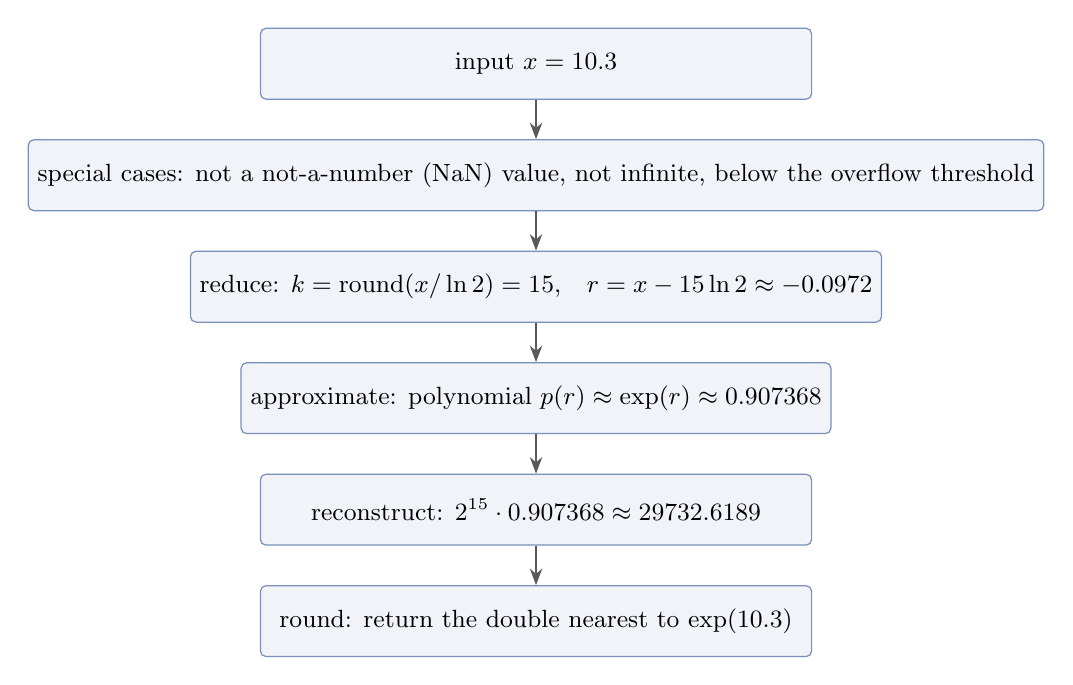
\begin{tikzpicture}[node distance=0.5cm]
    \node (inp)  [flowbox] {input $x = 10.3$};
    \node (spec) [flowbox, below=of inp]
    {special cases: not a not-a-number (NaN) value, not infinite, below the overflow threshold};
    \node (red)  [flowbox, below=of spec]
    {reduce: $k = \mathrm{round}(x / \ln 2) = 15$,\quad
        $r = x - 15\ln 2 \approx -0.0972$};
    \node (appr) [flowbox, below=of red]
    {approximate: polynomial $p(r) \approx \exp(r) \approx 0.907368$};
    \node (rec)  [flowbox, below=of appr]
    {reconstruct: $2^{15} \cdot 0.907368 \approx 29732.6189$};
    \node (rnd)  [flowbox, below=of rec]
    {round: return the double nearest to $\exp(10.3)$};

    \draw[arrow] (inp)  -- (spec);
    \draw[arrow] (spec) -- (red);
    \draw[arrow] (red)  -- (appr);
    \draw[arrow] (appr) -- (rec);
    \draw[arrow] (rec)  -- (rnd);
        \end{tikzpicture}
        \caption{The four-stage pipeline on a concrete call. The reduction
        moves the power-of-two scale into the integer $k$, the polynomial only
        ever sees the small residual $r$, and the reconstruction puts the scale
        back.}
        \label{fig:pipeline}
        \Description{Flowchart of an exp call passing through special-case checks, reduction, polynomial approximation, reconstruction, and final rounding.}
    \end{figure}

% -----------------------------------------------------------------------


    \section{The core problem}
    \label{sec:core}

    A handful of operations are \emph{correctly rounded} on every conforming
    platform: addition, subtraction, multiplication, division, square root, and
    the fused multiply-add (FMA) operation are required by the Institute of Electrical and Electronics Engineers (IEEE)~754 standard to behave as if the exact result
    were computed to infinite precision and rounded once~\cite{ieee}.
    Almost everything else cannot be handled that way.

    \texttt{exp}, \texttt{log}, \texttt{sin}, \texttt{cos}, \texttt{atan},
    \texttt{pow}, \texttt{tgamma}, and the rest are transcendental or
    algebraic-but-irrational. For almost every representable input the exact
    value is irrational, so no finite sequence of additions, multiplications,
    divisions, and square roots produces it. An implementation can only
    compute a value close enough that it rounds to the right answer in the
    target format.

    Implementing such a function is an engineering process with four recurring
    stages~\cite{muller,handbook}:

    \begin{enumerate}
        \item \textbf{Argument reduction.}  Use mathematical identities to map
        the input into a small, well-behaved interval.
        \item \textbf{Approximation.}  Replace the true function by a polynomial
        whose error is small and bounded by a proof.
        \item \textbf{Reconstruction.}  Combine the approximation with information
        discarded during reduction to recover the full-range result.
        \item \textbf{Rounding.}  Deliver the result correctly (or faithfully\footnote{Faithful rounding means returning either the floating-point value immediately below the exact result or the one immediately above it. Correct rounding is stricter: it returns the value selected by the active rounding mode.})
        rounded in the target format, in every rounding mode the function supports.
    \end{enumerate}

    Even the familiar series do not make the direct approach viable. The Taylor
    series for sine converges for every real input, but a naive double-precision
    sum is not a usable implementation. For $x = 100$, the largest term of the
    series is about $1.1 \cdot 10^{42}$, while the final result lies in
    $[-1, 1]$. The leading 42 digits must cancel, and a double carries about
    16. Every useful digit is destroyed before the sum settles. Reduction
    keeps the polynomial on a small interval where nothing like this can
    happen.

    A full implementation is not needed to see the problem. Take the degree~13
    Taylor polynomial for sine and compare absolute error two ways: directly on
    the raw input, and as the kernel behind a reduction modulo $\pi/2$.

    \begin{table}[H]
        \centering
        \begin{tabular}{lcc}
            \toprule
            Input & \shortstack{Direct Taylor\\absolute error}   & \shortstack{Reduced-kernel\\absolute error}  \\
            \midrule
            $x = 1$ & $7.6 \cdot 10^{-13}$  & below $6.7 \cdot 10^{-10}$ \\
            $x = 10$ & $5.5 \cdot 10^{2}$  & below $6.7 \cdot 10^{-10}$ \\
            $x = 100$ & $1.6 \cdot 10^{16}$  & below $6.7 \cdot 10^{-10}$ \\
            \bottomrule
        \end{tabular}
    \end{table}

    Both numeric columns are absolute-error magnitudes. The reduced-column
    entries assume an accurate reducer and quote the certified bound of the same
    polynomial on $[-\pi/2, \pi/2]$. For a small input such as $x = 1$, the direct
    Taylor polynomial can already be more accurate than this coarse reduced-path
    bound. That does not change the reason for reduction: it gives one uniform
    interval where the polynomial has a controlled worst-case error, including
    inputs such as $x = 10$ and $x = 100$ where the unreduced polynomial fails
    completely. The direct column shows that cost for $x = 10$: error around
    $550$, while the true result never leaves $[-1, 1]$.

    Stages~1, 3, and~4 are function-specific algebra and careful
    floating-point bookkeeping. Stage~2 is where Sollya is used.

% -----------------------------------------------------------------------


    \section{Polynomial approximation}

    Once reduction has made the interval small, the usual replacement is a
    polynomial. It uses operations the hardware already provides, fits Horner\footnote{Horner evaluation rewrites a polynomial as nested multiply-add steps, for example $c_0 + x(c_1 + x(c_2 + \cdots))$. It is compact and maps well to FMA-heavy code.} or
    FMA-heavy evaluation schemes, and gives analysis tools something finite to
    bound.

    Writing down a polynomial is not the hard part. The hard part is choosing
    coefficients that spend the available degree on the whole interval, under the
    same error model that the final implementation will claim.

% -----------------------------------------------------------------------


    \section{Taylor approximation}

    A Taylor series centered at zero has the form
    \[
        f(x) = \sum_{k=0}^{\infty} \frac{f^{(k)}(0)}{k!}\, x^k.
    \]
    Truncating at degree $n$ gives a polynomial whose error is smallest at $x = 0$
    and grows toward the interval edges.

    That behavior comes from what the Taylor polynomial is allowed to know. It
    uses the value of $f$ and the first $n$ derivatives at the center, and it has
    no direct information about the rest of the interval. The fit is excellent
    near the center and has nothing holding it down near the endpoints, which is
    where the worst-case error accumulates.

    \begin{figure}[tbp]
        \centering
        \begin{tikzpicture}
            \begin{semilogyaxis}
                [
                width=0.7\linewidth, height=5cm,
                xlabel={degree},
                ylabel={supremum error on $[-\pi/2,\,\pi/2]$},
                grid=both, grid style={gray!30},
                xtick={1,3,5,7,9,11,13},
                ymin=1e-10, ymax=2,
                mark size=2pt,
                ]
                \addplot[color=figblue, mark=*, thick]
                table[x=degree, y=abs_sup_error]
                    {\approxdata{sin_taylor_degree_error.dat}};
            \end{semilogyaxis}
        \end{tikzpicture}
        \caption[Supremum absolute error of odd Taylor sine polynomials]{Supremum\protect\footnotemark{} absolute error of odd Taylor sine polynomials on
            $[-\pi/2,\pi/2]$ as a function of degree, certified with Sollya's
            \texttt{supnorm}. Adding terms reduces the error, but the distribution
            is worst-case at the interval endpoints.}
        \Description{Semilog plot showing the supremum absolute error of odd Taylor sine polynomials falling as degree increases.}
    \end{figure}
    \footnotetext{The supremum of an error over an interval is the largest error attained anywhere on that interval. In this guide, ``supremum error'' means the worst-case error bound over the stated input range.}

    Small spot checks are misleading here. A Taylor polynomial can pass the
    inputs near its center and still lose badly at the endpoints, so the interval
    supremum is the quantity that drives the design.

    Once the degree and storage formats are fixed, the usual next tool is minimax
    approximation.

% -----------------------------------------------------------------------


    \section{Minimax approximation}

    A minimax polynomial is chosen by the worst input on the interval: it minimizes
    the largest error, not the average error and not the error near one favored
    point.

    That matches the usual libm objective. The implementation must answer any
    input in the reduced interval, so a polynomial that spends all its accuracy at
    the center is usually the wrong object.

    Minimax comes in flavors. The error being minimized can be absolute,
    relative, or weighted by any positive function, and the search can be
    constrained, for example to odd powers only or with the leading
    coefficient pinned to an exact value. Production kernels almost always
    use the relative or weighted form, for unit in the last place (ULP) accuracy reasons covered in
    Section~\ref{sec:relabs}, and the constrained forms appear whenever
    symmetry or an exact leading term is part of the design.

    One useful mental model is a fixed budget. A degree $n$ polynomial has
    $n + 1$ coefficients. Lowering the error in one part of the interval usually
    raises it somewhere else. At the optimum, the remaining peaks have been
    balanced against each other: they reach the same magnitude and alternate in
    sign. This is the equioscillation pattern.\footnote{Equioscillation means the largest positive and negative errors alternate and have nearly the same magnitude. It is the visual signature expected from a minimax fit in the appropriate approximation space.}

    For an unconstrained degree $n$ polynomial in the usual Chebyshev setting,\footnote{Here ``Chebyshev setting'' means uniform, worst-case approximation on an interval using the supremum norm.}
    the best minimax approximation has an error curve that reaches its maximum
    size at least $n + 2$ times, with alternating signs~\cite{muller}.
    Constrained spaces have their own alternation conditions, but the review
    heuristic is the same: the largest errors should be balanced rather than
    concentrated in one spike.

    Use the pattern during review. One dominant spike with long quiet regions is
    a warning sign. Balanced alternating peaks do not prove the whole
    implementation, but they are evidence that the approximation is using its degree
    for the intended interval.

    Taylor and minimax spend the same degree in very different places.
    Figure~\ref{fig:minimaxcompare} shows the difference directly. Both
    polynomials have degree~5 and cover the same interval. The Taylor error
    climbs monotonically to $4.5 \cdot 10^{-3}$ at the endpoints. The minimax
    error never exceeds $6.8 \cdot 10^{-5}$, about 67~times smaller, and shows
    the equal alternating-error pattern the theorem predicts. Because this sine fit
    uses an odd symmetric polynomial space, the visible contact points come in
    symmetric pairs; the unconstrained $n+2$ count should be read as a lower bound,
    not as the exact number a symmetric plot must display.

    \begin{figure}[tbp]
        \centering
        \begin{tikzpicture}
            \begin{axis}
                [
                width=0.48\linewidth, height=5.2cm,
                title={degree 5 Taylor},
                xlabel={$x$}, ylabel={signed error},
                grid=both, grid style={gray!30},
                ]
                \addplot[color=figblue, thick]
                table[x=x, y=taylor_error]
                    {\approxdata{sin_minimax_error.dat}};
            \end{axis}
        \end{tikzpicture}%
        \hfill
        \begin{tikzpicture}
            \begin{axis}
                [
                width=0.48\linewidth, height=5.2cm,
                title={degree 5 minimax},
                xlabel={$x$},
                grid=both, grid style={gray!30},
                ]
                \addplot[color=figblue, thick]
                table[x=x, y=minimax_error]
                    {\approxdata{sin_minimax_error.dat}};
            \end{axis}
        \end{tikzpicture}
        \caption{Signed error of two degree~5 approximations to $\sin(x)$ on
            $[-\pi/2,\pi/2]$. Note the scales: the Taylor peak is about 67~times
            taller, even though both polynomials have the same degree and cost the
            same to evaluate. The minimax curve equioscillates: its largest
            positive and negative errors are balanced across the interval. In the
            unconstrained degree-$5$ case the alternation theorem requires at least
            $n + 2 = 7$ contact points; the odd symmetric fit shown here has contacts
            in symmetric pairs.}
        \label{fig:minimaxcompare}
        \Description{Side-by-side signed-error plots comparing a degree 5 Taylor sine polynomial with a degree 5 minimax sine polynomial.}
    \end{figure}

% -----------------------------------------------------------------------


    \section{Remez}

    Remez exchange is the workhorse algorithm behind most of the minimax
    polynomials used in this style of implementation.

    Remez works backward from the equioscillation property. It guesses where the
    $n + 2$ worst-error points should sit, then solves a linear system for the
    unique polynomial whose error at exactly those points has equal magnitude and
    alternating sign. That polynomial is optimal for the guessed points, but its
    true error peaks may lie elsewhere. The algorithm then finds the actual
    extrema\footnote{An extremum is a local maximum or local minimum. Here the extrema are the peaks and valleys of the error curve.} of the error curve, moves the guessed points there, and repeats. When
    the true peaks stop moving, the error curve has the minimax shape and the loop
    stops~\cite{muller}. Convergence is usually fast once the reference points sit
    near their final positions, though hard functions and poor starting points can
    make the early iterations wander.

    \begin{figure}[H]
        \centering
        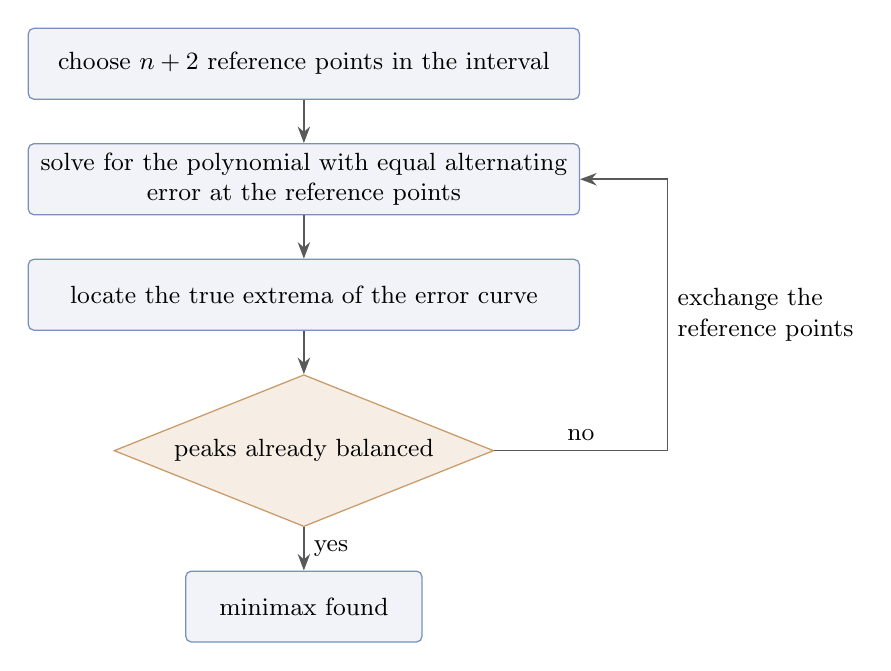
\begin{tikzpicture}[node distance=0.55cm]
    \node (init) [flowbox] {choose $n + 2$ reference points in the interval};
    \node (solve) [flowbox, below=of init]
    {solve for the polynomial with equal alternating\\error at the
    reference points};
    \node (find) [flowbox, below=of solve]
    {locate the true extrema of the error curve};
    \node (dec)  [decisionbox, below=of find] {peaks already balanced};
    \node (done) [flowbox, minimum width=3cm, below=of dec] {minimax found};

    \draw[arrow] (init)  -- (solve);
    \draw[arrow] (solve) -- (find);
    \draw[arrow] (find)  -- (dec);
    \draw[arrow] (dec) -- node[right, font=\small]{yes} (done);
    \draw[arrow] (dec.east) -- node[above, font=\small]{no}
    ++(2.2,0) |- node[pos=0.25, right, font=\small, align=left]
        {exchange the\\reference points} (solve.east);
        \end{tikzpicture}
        \caption{The Remez exchange loop. Each pass pins the error at the
        current reference points, then checks whether the real peaks agree.}
        \Description{Visual aid for the concept described in the caption.}
    \end{figure}

    In Sollya this exploratory step is the \texttt{remez} command.

    Remez is still one abstraction too high for source code. Its coefficients are
    real numbers. The implementation has \texttt{float}, \texttt{double},
    \texttt{long}~\texttt{double}, fixed-width constants, or explicit expansions
    such as double-double pairs.\footnote{A double-double value stores one number as the unevaluated sum of two doubles, usually a leading part and a correction part. It gives more significand precision but not the full exponent range of a wider binary format.}

    Use the real-coefficient result to choose the shape and degree. Do not treat
    it as the final source polynomial.

% -----------------------------------------------------------------------


    \section{Coefficients must fit the machine}

    Hand-rounding a real-coefficient minimax polynomial is a common way to lose
    the property that made the polynomial useful. The rounded version can have a
    different error shape, and the bound can grow enough to miss the target~\cite{muller}.

    Minimax optima are sensitive. The search tuned every coefficient against
    every other coefficient to make the peaks equal. Rounding each coefficient
    independently perturbs the error curve by amounts comparable to the gap the
    optimization fought for, and the perturbations do not cancel reliably.
    Finding the best machine-representable polynomial is its own optimization
    problem, separate from rounding the real-coefficient one.

    Sollya's \texttt{fpminimax} command addresses this problem.

    \texttt{fpminimax} searches for a near-minimax polynomial whose coefficients
    are already constrained to the requested
    formats~\cite{brisebarre2007,handbook}.

    In practice, keep the split simple:

    \begin{table}[tbp]
        \centering
        \begin{tabular}{ll}
            \toprule
            Step               & Use                                        \\
            \midrule
            \texttt{remez}     & Explore the real-coefficient approximation \\
            \texttt{fpminimax} & Generate coefficients for source code      \\
            \bottomrule
        \end{tabular}
    \end{table}

    \begin{pitfall}{constants that are almost right}
        Do not hand-round production coefficients unless the rounded polynomial is
        checked again. A bad constant can ruin a good algorithm. A decimal
        literal that looks harmless may round differently than the value Sollya
        produced. Prefer hexadecimal constants when the value is meant to be
        exact in the target format.
    \end{pitfall}

% -----------------------------------------------------------------------


    \section{Absolute error and relative error}
    \label{sec:relabs}

    Pick the error model before generating coefficients.

    Absolute error is:
    \[ |p(x) - f(x)| \]

    Relative error is:
    \[ \left|\frac{p(x)}{f(x)} - 1\right| \]

    ULP-based accuracy pushes the choice toward relative error. ULP size changes
    with the magnitude of the result~\cite{handbook}, so the same absolute error
    can be harmless in one binade\footnote{A binade is the interval between two consecutive powers of two, such as $[1,2)$ or $[2,4)$. Floating-point spacing is constant inside one binade and changes at binade boundaries.} and disastrous in another.

    Figure~\ref{fig:ulpspacing} shows why. The figure uses a toy format with three significand\footnote{The significand is the precision-carrying part of a floating-point number. In binary64, it has 53 bits including the implicit leading bit for normal values.} bits.

    \begin{figure}[H]
        \centering
        \begin{tikzpicture}[xscale=3.4]
    \draw[-{Stealth}] (0.85,0) -- (4.35,0);
    \foreach \x in {1,1.125,...,2} \draw (\x,-0.07) -- (\x,0.07);
    \foreach \x in {2.25,2.5,...,4.01} \draw (\x,-0.07) -- (\x,0.07);
    \foreach \x in {1,2,4} \node[below=3pt, font=\small] at (\x,0) {$\x$};
    \draw[decorate, decoration={brace, amplitude=4pt}]
    (1.5,0.14) -- (1.625,0.14)
    node[midway, above=5pt, font=\small] {ulp $= 1/8$};
    \draw[decorate, decoration={brace, amplitude=4pt}]
    (3,0.14) -- (3.25,0.14)
    node[midway, above=5pt, font=\small] {ulp $= 1/4$};
        \end{tikzpicture}
        \caption{Representable values of a toy binary format with three
        significand bits. The spacing is constant inside each binade and
        doubles at every power of two. Real formats behave the same way with
        much finer spacing.}
        \label{fig:ulpspacing}
        \Description{Visual aid for the concept described in the caption.}
    \end{figure}

    Floating-point values are not evenly spaced. Within one binade, the interval
    between consecutive powers of two, the spacing is constant. At each power of
    two it doubles. A fixed absolute error therefore costs a different number of
    ULPs depending on where the result lands: in double precision, an error of
    $2^{-55}$ is an eighth of an ULP for a result near~1 and 128~ULPs for a result
    near $2^{-10}$. Relative error divides that scale out. A relative bound
    translates into a roughly uniform ULP bound at every magnitude, which is why it
    is the usual target when the function's result spans many binades.

    Relative error still has traps. Near a zero of $f$, the division by $f(x)$
    can dominate the measurement instead of describing the implementation risk.
    In that case, change the kernel. Section~\ref{sec:kernel} lists the usual
    transforms.

    Two more regions deserve care. When the result is subnormal,\footnote{A subnormal is a nonzero floating-point value whose magnitude is smaller than the smallest normal value. Subnormals fill the gap between zero and the normal range, but with reduced precision.} the format
    quantizes more coarsely than the relative model assumes, so relative
    error and ULP distance part ways there. When the result sits near the
    overflow threshold, a relative polynomial bound says nothing about
    whether the rounded result becomes infinity. Both regions belong to the
    special-case plan, not to the polynomial.


    \begin{checkpoint}
        Mini exercise: make the ULP scale concrete. Suppose a kernel has a fixed
        absolute error of $2^{-55}$.
        \begin{enumerate}
            \item Near a result of magnitude~1, how many ULPs is that?
            \item Near a result of magnitude $2^{-10}$, how many ULPs is that?
            \item In one sentence, explain why this pushes many kernels toward
            relative or weighted error instead of plain absolute error.
        \end{enumerate}
    \end{checkpoint}

% -----------------------------------------------------------------------


    \section{Sollya}

    Use Sollya for the approximation work in this guide: coefficient generation,
    quick exploration, and certified interval checks~\cite{sollyapaper}.

    In this guide, Sollya is used for the following jobs:

    \begin{table}[H]
        \centering
        \caption{Sollya commands used in this guide.}
        \begin{tabular}{ll}
            \toprule
            Task                                          & Sollya command                       \\
            \midrule
            Estimate the needed degree                    & \texttt{guessdegree}                 \\
            Compute a real-coefficient minimax polynomial & \texttt{remez}                       \\
            Compute machine-format coefficients           & \texttt{fpminimax}                   \\
            Quickly estimate worst-case error             & \texttt{dirtyinfnorm}                \\
            Compute a safer error bound                   & \texttt{infnorm} or \texttt{supnorm} \\
            Print constants for source code               & \texttt{display = hexadecimal}       \\
            Print Horner form                             & \texttt{horner}                      \\
            Print expanded form                           & \texttt{canonical}                   \\
            \bottomrule
        \end{tabular}
    \end{table}

    \subsection{Running Sollya}

    A script run looks like this:
    \begin{lstlisting}[style=shell]
sollya docs/approximating_functions/sollya/script.sollya
    \end{lstlisting}

    Start scripts like this:
    \begin{lstlisting}[style=sollya]
prec = 200!;
display = hexadecimal!;
    \end{lstlisting}


    The precision setting controls Sollya's working precision. It should be
    higher than the target format. For double coefficients, 200 bits is a
    reasonable starting point.

    Print production constants in hexadecimal. That gives C++ the same
    floating-point value Sollya printed. A decimal spelling can add a second
    rounding step.

% -----------------------------------------------------------------------


    \section{A small Sollya example}
    \label{sec:sollyaexample}

    For a first Sollya run, start after range reduction. Assume the input has
    already been reduced from $\exp(x)$ to $\exp(r)$ with $r$ close to zero.

    The usual shape is:
    \[ \exp(x) = 2^k \exp(r) \]
    where $r$ lies in an interval such as:
    \[ \left[-\frac{\ln(2)}{2},\ \frac{\ln(2)}{2}\right] \]

    The following script is intentionally small enough to run as printed:
    \begin{lstlisting}[style=sollya]
prec = 200!;

f = exp(x);
I = [-log(2) / 2; log(2) / 2];

print("suggested degree for 1b-53 relative:");
guessdegree(f, I, 1b-53);

p = fpminimax(f, 11, [|D, D, D, D, D, D, D, D, D, D, D, D|], I, relative);

print("coefficients:");
display = hexadecimal!;
for i from 0 to 11 do coeff(p, i);
display = decimal!;

eps_fast = dirtyinfnorm(p / f - 1, I);
print("quick relative error estimate:", eps_fast);

eps_cert = supnorm(p, f, I, relative, 1b-40);
print("certified relative error:", eps_cert);
    \end{lstlisting}

    The format list \texttt{[|D, D, \ldots|]} names the storage format of
    each coefficient from degree~0 upward, one entry per coefficient, D
    meaning double. Mixed lists are common in real kernels, for example a
    double-double pair for the leading coefficients and plain doubles for
    the tail.

    Expected output, with the long decimals shortened:

    \begin{lstlisting}[style=output]
suggested degree for 1b-53 relative:
[11;11]
coefficients:
0x1p0
0x1p0
0x1.000000000000bp-1
0x1.5555555555511p-3
0x1.55555555502a1p-5
0x1.1111111122322p-7
0x1.6c16c1852b7bp-10
0x1.a01a014761f6ep-13
0x1.a01997c89e6bp-16
0x1.71dee623fde67p-19
0x1.28af3fca7ab0cp-22
0x1.ade156a5dbe77p-26
quick relative error estimate: 4.0961995708e-18
certified relative error: [4.0961995708e-18; 4.0961995712e-18]
    \end{lstlisting}

    Read the output as a set of design checks.  \texttt{guessdegree} reports
    that degree~11 is the first degree that can reach $2^{-53}$ on this interval,
    so the script asks for that degree rather than guessing. The first coefficients
    sit on the Taylor values $1, 1, 1/2, 1/6$ to within a few ULPs, which is
    a good sanity check. The certified bound is an enclosure, not a point
    value: the true supremum lies inside the printed interval, so quote its
    upper end, $4.1 \cdot 10^{-18} \approx 2^{-57.8}$. Read
    $-\log_2(\text{error})$ as a rough count of correct bits. Here the bound is
    about $2^{-57.8}$, so the polynomial has about 58 bits of approximation
    margin before reduction, evaluation, and reconstruction spend any of it.

    A packaged copy of this script ships as
    \path{docs/approximating_functions/sollya/exp_small_fpminimax.sollya}.

    That bound covers only the exact polynomial approximation to $\exp(r)$ on
    that interval. A complete \texttt{exp} still has to prove the reducer,
    rounded evaluation, reconstruction, special cases, and final rounding.


    \begin{checkpoint}
        Mini exercise: spend the bit budget. The polynomial bound above is about
        $2^{-57.8}$ relative. Suppose the reducer, evaluation scheme, and
        reconstruction together spend about 5 bits of margin.
        \begin{enumerate}
            \item About how many bits of margin remain before the binary64
            half-ULP target?
            \item Would you call that comfortable, tight, or already over budget?
        \end{enumerate}
    \end{checkpoint}

% -----------------------------------------------------------------------


    \section{Choosing the kernel}
    \label{sec:kernel}

    After reduction, the implementation usually works with a smaller kernel rather
    than the public function directly.


    For $\sin(x)$, the kernel may be $\sin(r)$.

    For small $x$, it may be better to approximate $\sin(r)$ divided by $r$.

    For \texttt{log1p}, it may be better to approximate $\log(1+r)$
    divided by $r$.

    For $\mathrm{expm1}(x)$, it may be better to approximate
    $\mathrm{expm1}(r)$ divided by $r$.

    A useful kernel removes cancellation, keeps the relative error model stable near
    zero, and can reduce the polynomial degree.

    Do the algebra before asking Sollya for coefficients.

    What should be small after reduction, and what should be exact? That choice
    often determines the kernel.

    \subsection{Small-input transforms}
    \begin{align*}
        \log(1+x) &= x \cdot \frac{\log(1+x)}{x} \\[4pt]
        \exp(x)-1  &= x \cdot \frac{\exp(x)-1}{x} \\[4pt]
        \sin(x)    &= x \cdot \frac{\sin(x)}{x} \\[4pt]
        \cos(x)    &= 1 - 2\sin^2\!\left(\tfrac{x}{2}\right)
    \end{align*}

    These are mainly small-input tools. By factoring out the term that causes
    cancellation or unstable relative error, they leave a smoother quotient or a
    reconstruction identity that preserves more useful bits.

    The quotient forms rely on removable singularities.\footnote{A removable singularity is a point where a formula is undefined, but the limit exists. The function can be extended by assigning that limiting value.}  $\sin(x)/x$ is undefined
    at $x = 0$, but its limit there is 1, and the function extended with that value
    is smooth across the whole interval. That extended function is what the
    polynomial approximates, and Sollya handles the extension automatically. For
    quotient kernels like these, the production path usually does not divide by
    the small input. It approximates the removable extension and multiplies by
    the factored term during reconstruction, so the input $x = 0$ flows through
    as $x \cdot p(0) = 0$ with the correct sign.

    The identity must still be checked on the target interval and under the
    target rounding policy. None of these forms is automatically best on every
    interval.

% -----------------------------------------------------------------------


    \section{Worked example: a small sine kernel}

    \begin{tcolorbox}[colback=blue!5, colframe=blue!30, title={Start here for hands-on work}]
        If you want to run Sollya and follow code in order, begin with
        Section~\ref{sec:setup} and Section~\ref{sec:target}.
        Skim Section~\ref{sec:core} through Section~\ref{sec:relabs} first if the
        approximation vocabulary is new.
    \end{tcolorbox}

    The first kernel is deliberately small, so all of the moving parts stay visible:
    \[
        \texttt{sin\_small}(x) \approx \sin(x) \quad \text{for } |x| \le \tfrac{1}{16}
    \]

    It is not a public \texttt{sin}. There is no quadrant logic, no large-input
    reduction, and no special-case table. The restriction keeps the kernel small
    enough to audit on one screen.

    \subsection{Set up Sollya}
    \label{sec:setup}

    Only Sollya is required for the worked examples. Install it once, then run
    the companion scripts from the repository root:

    \begin{lstlisting}[style=shell]
# macOS
brew install sollya

# Debian/Ubuntu
sudo apt update
sudo apt install sollya

sollya docs/approximating_functions/sollya/sin_small_error.sollya
    \end{lstlisting}

    On Windows, use Ubuntu under the Windows Subsystem for Linux (WSL). From an
    Administrator PowerShell prompt, install Ubuntu:

    \begin{lstlisting}[style=shell]
wsl --install -d Ubuntu
    \end{lstlisting}

    Restart if Windows asks. Then open Ubuntu from the Start menu, create the
    Linux user when prompted, and run the Debian/Ubuntu commands above inside
    that Ubuntu shell. Keeping the checkout under the Linux home directory, for
    example \path{~/src/ccmath}, usually gives fewer path and filesystem surprises
    than running the scripts from \path{/mnt/c/...}.

    The expected output after each script was produced with Sollya~8.0. Numbers
    certified by \texttt{supnorm} are reproducible across versions, although
    incidental formatting may differ. The build script
    \path{docs/approximating_functions/build.sh} reruns the same scripts when
    the guide PDF is rebuilt. Multiple Precision Floating-Point Reliable Library (MPFR), Gappa, Rocq, and SageMath are useful later for
    validation, but they are not required to follow the examples here.

    \subsection{Specify the target}
    \label{sec:target}

    \begin{center}
        \begin{tabular}{ll}
            Target:                           & $f(x) = \sin(x)$ \\[3pt]
            Input interval:                   & $x \in \left[-\dfrac{1}{16},\, \dfrac{1}{16}\right]$ \\[8pt]
            Output type:                      & \texttt{double} \\[3pt]
            Accuracy target for this example: & well below 1~ULP on the stated interval under round-to-nearest \\
        \end{tabular}
    \end{center}

    \subsection{Choose the kernel}

    Directly approximating $\sin(x)$ works on this interval, but the odd symmetry
    is useful. Since $\sin(x)$ is odd:
    \[
        \sin(x) = x q(x^2)
    \]
    where:
    \[
        q(z) = \frac{\sin(\sqrt{z})}{\sqrt{z}}
    \]

    At $z = 0$, read $q$ by its removable extension, $q(0) = 1$.
    Near zero, $q(z)$ is smooth and close to~1.

    The implementation will compute:
    \[
        z = x^2
    \]
    and:
    \[
        \sin(x) \approx x\,p(z)
    \]
    where $p$ approximates $q$.

    \subsection{Pick a simple polynomial}

    For the teaching version, Taylor coefficients make the arithmetic easy to
    recognize:
    \[
        \sin(x) = x - \frac{x^3}{6} + \frac{x^5}{120} - \frac{x^7}{5040} +
        \frac{x^9}{362880} + \cdots
    \]

    Factoring out $x$ gives:
    \[
        \sin(x) = x\!\left(1 - \frac{z}{6} + \frac{z^2}{120} - \frac{z^3}{5040} +
                         \frac{z^4}{362880} + \cdots\right)
    \]
    where $z = x^2$.

    Production code would use \texttt{fpminimax} coefficients here. Taylor values
    keep the arithmetic recognizable while the workflow is new, and
    Section~\ref{sec:sinprod} runs \texttt{fpminimax} on this same kernel so the two
    can be compared. Either way, Sollya checks the error of whatever polynomial
    actually ships.

    \subsection{Check the approximation in Sollya}

    Now bound the error on the exact interval the kernel promises:
    \begin{lstlisting}[style=sollya]
prec = 200!;
display = hexadecimal!;

I = [-1/16; 1/16];

p = x * (
    0x1.0000000000000p+0
  + x^2 * (
      -0x1.5555555555555p-3
    + x^2 * (
        0x1.1111111111111p-7
      + x^2 * (
          -0x1.a01a01a01a01ap-13
        + x^2 * 0x1.71de3a556c734p-19
      )
    )
  )
);

abs_err = supnorm(p, sin(x), I, absolute, 1b-80);
rel_err = supnorm(p, sin(x), I, relative, 1b-80);

display = decimal!;
print("absolute error:", abs_err);
print("relative error:", rel_err);
    \end{lstlisting}

    Expected output, shortened:

    \begin{lstlisting}[style=output]
absolute error: [3.6826560686e-21; 3.6826560686e-21]
relative error: [5.8960875588e-20; 5.8960875588e-20]
    \end{lstlisting}

    So the certified approximation error of this polynomial is
    $3.69 \cdot 10^{-21}$ absolute and $5.90 \cdot 10^{-20} \approx 2^{-63.9}$
    relative on the stated interval. Both numbers reappear in the worked
    budget of Section~\ref{sec:sinproof}.

    The familiar series does not justify the code. The checked interval and the
    reported bound do.

    \subsection{Implement the kernel}

    Horner form gives the C++ kernel without changing the coefficient order:
    \Needspace{18\baselineskip}
    \begin{lstlisting}[style=cpp]
[[nodiscard]] constexpr double sin_small(double x) noexcept
{
    const double z = x * x;

    const double p =
        (((0x1.71de3a556c734p-19 * z
         - 0x1.a01a01a01a01ap-13) * z
         + 0x1.1111111111111p-7) * z
         - 0x1.5555555555555p-3) * z
         + 0x1.0000000000000p+0;

    return x * p;
}
    \end{lstlisting}

    This kernel does not defend its interval. Its caller must supply values with
    $|x| \le 1/16$. In a real internal path, the surrounding reducer owns that
    precondition, and the tests should call the kernel only through reduced
    inputs or explicit reduced-interval cases.

    The kernel is plain C++17. Every number quoted for it in this guide was
    measured with \texttt{-O2} and no fast-math flags.
    Section~\ref{sec:compiler} explains why the flags are part of the claim.

    \subsection{Test the kernel}

    For this restricted kernel, useful tests include:

    \begin{enumerate}
        \item $x$ equals~$0$
        \item $x$ equals the interval endpoints
        \item several values near the endpoints
        \item positive and negative inputs with matching signs
        \item comparison against MPFR or another high-precision oracle\footnote{An oracle is an independent reference calculation used to check the implementation. In this guide the oracle is usually MPFR run at higher precision.}
    \end{enumerate}

    For round-to-nearest tests, compare the returned bit pattern or ULP distance.
    Printed decimal text is the wrong target.

    Example values:
    \[
        0,\quad \frac{1}{1024},\quad -\frac{1}{1024},\quad \frac{1}{32},\quad
        -\frac{1}{32},\quad \frac{1}{16},\quad -\frac{1}{16}
    \]

    Keep the endpoints in the test set. The approximation was proved only on that
    interval. If a later change expands the interval to $[-1/8,1/8]$, the proof
    and tests must be redone.

    ULP distance is worth implementing once and reusing everywhere. The
    trick is to map doubles onto the integers so that consecutive finite
    doubles map to consecutive integers:

    \begin{lstlisting}[style=cpp]
std::int64_t ulp_order(double v)
{
    std::int64_t bits;
    std::memcpy(&bits, &v, sizeof bits);
    return bits >= 0 ? bits : INT64_MIN - bits;
}

std::int64_t ulp_distance(double a, double b)
{
    const std::int64_t d = ulp_order(a) - ulp_order(b);
    return d < 0 ? -d : d;
}
    \end{lstlisting}

    The ordering works because IEEE doubles with the same sign already compare like
    integers bit-for-bit. The negative branch folds the other half of the line into
    the same order. A distance of 0 means correctly rounded against the oracle, and
    a distance of 1 means the adjacent double, which is the faithful-rounding
    criterion.

    A complete oracle harness using this, with MPFR as the reference, ships
    as \path{docs/approximating_functions/cpp/sin_small_check.cpp}. Build and
    run it from the repository root:
    \begin{lstlisting}[style=shell]
c++ -std=c++17 -O2 docs/approximating_functions/cpp/sin_small_check.cpp \
    -lmpfr -lgmp -o sin_small_check && ./sin_small_check
    \end{lstlisting}
    It sweeps the listed special values plus a dense grid. Its output on this
    kernel:

    \begin{center}
        \begin{tabular}{@{}ll@{}}
            \texttt{inputs tested:}     & \texttt{200001}                \\
            \texttt{correctly rounded:} & \texttt{162160}                \\
            \texttt{max ULP distance:}  & \texttt{1}                     \\
            \texttt{worst input:}       & \texttt{-0x1.fffeb074a771dp-5}
        \end{tabular}
    \end{center}

    On that grid, the kernel is faithful everywhere and correctly rounded for
    81~percent of the tested inputs. Its worst input is effectively an endpoint case, which is where this error
    curve is largest. A useful status table records those measurements alongside
    the proof bounds; the polynomial bound alone is not enough.

    \begin{figure}[H]
        \centering
        \begin{tikzpicture}
            \begin{axis}
                [
                width=0.7\linewidth, height=5.5cm,
                xlabel={$x$},
                ylabel={absolute error},
                grid=both, grid style={gray!30},
                xmin=-0.065, xmax=0.065,
                ]
                \addplot[color=figblue, thick]
                table[x=x, y=abs_error]
                    {\approxdata{sin_small_error.dat}};
            \end{axis}
        \end{tikzpicture}
        \caption{Absolute error of the small sine teaching polynomial on
            $[-1/16,1/16]$, sampled in Sollya at high working precision. Double
            arithmetic cannot even measure errors this small directly, which is why
            the curve comes from the script and not from a C++ harness.}
        \Description{Visual aid for the concept described in the caption.}
    \end{figure}

    \subsection{A production polynomial for the same kernel}
    \label{sec:sinprod}

    The Taylor coefficients were only for inspection. For the same degree,
    interval, and storage format, \texttt{fpminimax} produces the following
    coefficients, from
    \path{docs/approximating_functions/sollya/sin_small_fpminimax.sollya}.
    A direct request fails here: asking \texttt{fpminimax} for an odd
    polynomial against $\sin$ with relative error degenerates, because the
    odd basis is not a Chebyshev system\footnote{A Chebyshev system is a set of basis functions with enough structure for the usual minimax alternation theory to apply cleanly. If the chosen basis is not one for the weighted problem, Remez-style fitting can degenerate or fail.} for that weighted problem. The
    usual workaround is to fit the transformed kernel $\sin(x)/x$ with even
    monomials\footnote{A monomial is a single power term such as $1$, $x^2$, or $x^4$. Even monomials use only even powers.} instead, then multiply by $x$ in the implementation:

    \begin{lstlisting}[style=sollya]
I = [0; 1/16];
Icheck = [-1/16; 1/16];

q = fpminimax(sin(x)/x, [|0, 2, 4, 6, 8|], [|D, D, D, D, D|], I, relative);
p = x * q;
    \end{lstlisting}

    Expected output:

    \begin{lstlisting}[style=output]
coefficients of q, so that sin(x) ~ x * q(x^2):
  q0 = 0x1p0
  q2 = -0x1.5555555555555p-3
  q4 = 0x1.111111110f491p-7
  q6 = -0x1.a01a00e16af3ep-13
  q8 = 0x1.71c24233f1bafp-19
certified absolute error: [5.1436720042e-23; 5.1436720042e-23]
certified relative error: [2.0923182501e-21; 2.0923182501e-21]
    \end{lstlisting}

    Compare against the Taylor bounds from the check script. The degree and
    the evaluation cost have not changed, and the certified absolute error
    drops from $3.7 \cdot 10^{-21}$ to $5.1 \cdot 10^{-23}$, about 70~times.
    The first two coefficients match the Taylor values to the last bit. The
    lower ones drift away from them, because the optimizer adjusts the tail
    coefficients that the Taylor series ties to derivatives at zero.

    \subsection{Proving the evaluation error}
    \label{sec:sinproof}

    Sollya bounded the distance from the exact polynomial to $\sin$. The
    compiled kernel evaluates that polynomial in floating point, and every
    operation rounds. Gappa bounds this second distance. The proof file
    ships as
    \path{docs/approximating_functions/gappa/sin_small_eval.gappa} and
    its core mirrors the C++ operation for operation:

    \begin{lstlisting}[style=sollya]
x = rnd(x_);

z rnd= x * x;
p rnd= (((c9 * z + c7) * z + c5) * z + c3) * z + c1;
s rnd= x * p;

Mz = x * x;
Mp = (((c9 * Mz + c7) * Mz + c5) * Mz + c3) * Mz + c1;
Ms = x * Mp;

{ |x| <= 0x1p-4 -> |s - Ms| <= 0x1.02p-57 /\
  x in [0x1p-60, 0x1p-4] -> |s -/ Ms| <= 1b-52 }
    \end{lstlisting}

    Running \texttt{gappa} on the file succeeds silently, which is how Gappa
    reports a proof:
    \begin{lstlisting}[style=shell]
gappa docs/approximating_functions/gappa/sin_small_eval.gappa
    \end{lstlisting}
    The two goals say: the computed value $s$ sits within
    $2^{-56.99}$ of the exact polynomial value absolutely, and within
    $2^{-52}$ relatively on the positive half. The kernel is odd under
    exact negation, so the relative bound covers the negative half too.

    Now the budget for this kernel can be filled in with proven numbers
    instead of placeholders:

    \begin{table}[H]
        \centering
        \begin{tabular}{llll}
            \toprule
            Obligation & Tool & Absolute & Relative \\
            \midrule
            approximation, $p$ vs $\sin$ & Sollya \texttt{supnorm}
            & $3.7 \cdot 10^{-21}$ & $5.9 \cdot 10^{-20}$ \\
            evaluation, $s$ vs $p$ & Gappa
            & $7.0 \cdot 10^{-18}$ & $2^{-52}$ \\
            oracle agreement & MPFR harness
            & \multicolumn{2}{l}{max 1 ULP over 200001 inputs} \\
            \bottomrule
        \end{tabular}
    \end{table}

    The budget and the harness hit the same limit. Near the top of the
    interval, $\operatorname{ulp}(\sin x) = 2^{-57}$, and the proven
    evaluation-error bound is about one ULP. That is already larger than the
    half-ULP margin needed for a simple correct-rounding argument, so correct
    rounding cannot be guaranteed from this budget alone. The harness agrees:
    faithful everywhere on the grid, correctly rounded only 81~percent of the
    time. Tightening the proof to match the observed behavior would mean
    splitting the interval and proving scaled bounds piece by piece, which is
    where production correct-rounding proofs put most of their effort.

    \emph{Milestone.}  You can now take a smooth function on a small
    interval, generate a polynomial, certify its approximation error, bound
    its evaluation error, and check the result against an oracle. That is
    the complete inner loop of kernel work.

    \subsection{What this example leaves out}

    A full implementation still has additional obligations:

    \begin{enumerate}
        \item reduction for arbitrary finite inputs
        \item quadrant reconstruction
        \item handling of NaN and infinities
        \item signed-zero behavior
        \item directed rounding behavior
        \item large-input Payne-Hanek reduction
        \item validation against an oracle
        \item a recorded error budget for reduction, evaluation, and reconstruction
    \end{enumerate}

    Larger functions use the same loop, then add reduction, tables, multiple
    precision tiers, special cases, and harder rounding decisions.

    \begin{checkpoint}
        Before the next example, check the kernel you just built.
        \begin{enumerate}
            \item Why approximate $\sin(x)/x$ in $z = x^2$ instead of $\sin(x)$
            directly?
            \item The interval grows from $[-1/16, 1/16]$ to $[-1/8, 1/8]$. What
            must be redone?
            \item Why are the coefficients written in hexadecimal?
        \end{enumerate}
    \end{checkpoint}

% -----------------------------------------------------------------------


    \section{Advanced worked example: a small log2 core}
    \label{sec:log2}

    The next example adds the pieces missing from the small sine kernel: table
    reduction, a transformed kernel, split constants, and a polynomial on a small
    residual interval. A production-grade log with this structure,
    including its correct-rounding proof, is described in~\cite{dinechinlog}.
    Read that paper after this section and the structure will look familiar.

    This example is still not a full $\log_2$ implementation. It starts with the
    normalization step that every binary floating-point implementation can exploit.

    \subsection{Normalize the input}

    Before the table is useful, the input has to be split into the part that is
    already easy and the part that still needs approximation. For $\log_2$, powers
    of two are easy:
    \[ \log_2(2^e) = e. \]

    Every positive finite binary floating-point number is already stored in this
    shape: a significand carrying the useful bits, and a power-of-two exponent
    carrying the scale. After normalization, this can be written as:
    \[ x = m 2^e \]
    with:
    \[ m \in [1, 2). \]

    For example:
    \[ 13.25 = 1.65625 \cdot 2^3 \]
    so:
    \[ \log_2(13.25) = 3 + \log_2(1.65625). \]

    The exponent part is exact and needs no polynomial. The hard part is now only
    $\log_2(m)$, where $m$ always lies in the same fixed interval $[1,2)$. That
    fixed interval is what makes the reciprocal table useful.

    In C or C++, this split can be viewed as the job of \texttt{frexp}, although
    production kernels usually extract the exponent and significand bits directly
    so that boundary behavior is exact and easy to prove.

    The core below starts after that normalization step. It assumes the input has
    already been decomposed as:
    \[ x = m 2^e, \qquad m \in [1, 2). \]

    The full result is:
    \[ \log_2(x) = e + \log_2(m) \]

    The core computes the $\log_2(m)$ part.


    \begin{checkpoint}
        Mini exercise: normalize one input by hand. Write $0.15625$ as
        $m2^e$ with $m \in [1,2)$, then rewrite $\log_2(0.15625)$ as
        $e + \log_2(m)$.
    \end{checkpoint}

    \subsection{Choose the table reduction}

    Divide $[1, 2)$ into $B$ buckets. For a teaching version, use:
    \[ B = 16 \]

    For each bucket, choose a value $r_i$ close to the reciprocal of the bucket
    center. For an input mantissa\footnote{The mantissa is the scaled significand part of a floating-point value after separating out the power-of-two exponent. In modern IEEE terminology, this is usually called the significand.} $m$, compute:
    \[ u = m r_i - 1 \]

    If $r_i$ is well chosen, $u$ is small. The identity is:
    \[ m = \frac{1 + u}{r_i} \]
    so:
    \[ \log_2(m) = \log_2(1 + u) - \log_2(r_i) \]

    The table stores $r_i$ and a split form of $-\log_2(r_i)$.

    One split is:
    \[ -\log_2(r_i) = h_i + \ell_i \]

    The high part $h_i$ can be rounded to fewer bits so that the later addition
    with the exponent can be proved exact for the intended fast path. The low part $\ell_i$ carries the
    remaining bits.

    \subsection{What the table buys}

    The table exists to shrink the polynomial interval. With $B = 16$, a simple
    bucket-center choice leaves a residual roughly bounded by:
    \[ |u| \le \frac{1}{2B} \]

    This is the analytic bound for exact bucket-center reciprocals. Once $r_i$
    is rounded into the table format, the recorded residual interval must be
    recomputed from the generated table. More table bits shrink the interval
    that the polynomial has to cover.

    That is the trade: table entries cost memory and cache pressure, while a
    smaller residual can lower the degree or make the proof easier.

    \begin{figure}[H]
        \centering
        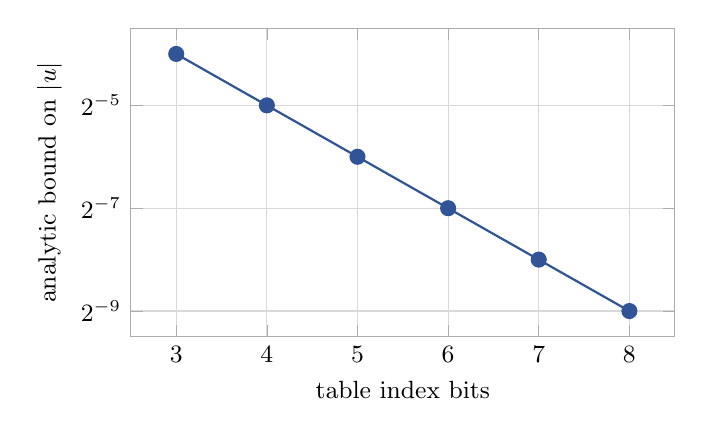
\begin{tikzpicture}
            \begin{axis}
                [
                width=0.7\linewidth, height=5.5cm,
                xlabel={table index bits},
                ylabel={analytic bound on $|u|$},
                ymode=log, log basis y=2,
                grid=both, grid style={gray!30},
                xtick={3,4,5,6,7,8},
                mark size=2.5pt,
                ]
                \addplot[color=figblue, mark=*, thick] coordinates {
                    (3, 0.0625)
                    (4, 0.03125)
                    (5, 0.015625)
                    (6, 0.0078125)
                    (7, 0.00390625)
                    (8, 0.001953125)
                };
            \end{axis}
        \end{tikzpicture}
        \caption{Analytic residual bound after one reciprocal table reduction.
        More table bits shrink the interval used by the polynomial.}
        \Description{Visual aid for the concept described in the caption.}
    \end{figure}
    \FloatBarrier

    \subsection{Approximate the residual function}

    After the table reduction, the remaining function is:
    \[ \log_2(1 + u) \]

    Since $u$ is small, approximate:
    \[ g(u) = \frac{\log_2(1 + u)}{u} \]

    Then:
    \[ \log_2(1 + u) \approx u\,p(u) \]

    Dividing by $u$ removes the zero at the origin. The resulting function
    $g(u)$ is smooth near zero and has value $1/\ln(2)$.

    A Sollya script for the polynomial looks like this:
    \begin{lstlisting}[style=sollya]
prec = 200!;
display = hexadecimal!;

U = [-1/32; 1/32];
g = log2(1 + x) / x;

p = fpminimax(g, 5, [|D...|], U, relative);

abs_err = supnorm(x * p, log2(1 + x), U, absolute, 1b-80);
rel_err = supnorm(p, g, U, relative, 1b-80);

print("absolute residual error:", abs_err);
print("relative kernel error:", rel_err);
print("polynomial:");
horner(p);
    \end{lstlisting}

    The script stops at the polynomial boundary. It does not validate
    table indexing, split constants, or the final addition with the exponent.
    A packaged copy ships as
    \path{docs/approximating_functions/sollya/log2_core_poly.sollya}.

    \subsection{Generate the table}

    Generate tables from the invariant, not from hand-edited rows. Each table row
    answers one local question: if $m$ lands in this bucket, what number should we
    multiply by to move it close to $1$, and what logarithm did that multiplication
    add that we must put back afterward?

    The bucket center is the representative input for the row. With $B$ buckets in
    $[1,2)$, row $i$ is centered at:
    \[ c_i = 1 + \frac{i + 1/2}{B}. \]
    For example, with $B=16$, the first bucket is centered at $1 + 1/32$.
    The table stores a rounded reciprocal of that center:
    \[ r_i = \mathrm{round}_D\!\left(\frac{1}{c_i}\right). \]
    Multiplying an input in the bucket by this reciprocal gives
    $m r_i = 1 + u$, with $u$ small. That is the whole point of the table: it turns
    $\log_2(m)$ into a small residual problem:
    \[
        \log_2(m) = \log_2(1 + u) - \log_2(r_i).
    \]

    The correction that must be added back is therefore:
    \[ a_i = -\log_2(r_i). \]

    A row is generated from those three facts:
    \begin{align*}
        c_i &= 1 + \frac{i + 1/2}{B} \\
        r_i &= \mathrm{round}_D\!\left(\frac{1}{c_i}\right) \\
        a_i &= -\log_2(r_i)
    \end{align*}

    The correction $a_i$ is then split into two stored pieces:
    \begin{align*}
        h_i &= \mathrm{round}_t(a_i) \\
        \ell_i &= \mathrm{round}_D(a_i - h_i)
    \end{align*}

    The high part $h_i$ is deliberately rounded to fewer bits. That makes the later
    addition $e + h_i$ easier to prove exact for the intended exponent range. The
    low part $\ell_i$ carries the small leftover correction. The final shape is
    therefore:
    \[
        \log_2(x) \approx (e + h_i) + (\ell_i + u p(u)).
    \]
    The split is not a new approximation idea. It is bookkeeping: put the large,
    easy-to-add correction in $h_i$, keep the leftover in $\ell_i$, and let the
    polynomial handle only the small residual $\log_2(1+u)$.

    Here $t$ is the chosen precision for the high part. It should be chosen so
    that the later addition with the exponent can be proved exact for the path
    being implemented.


    \begin{checkpoint}
        Mini exercise: walk one table row. Use $B = 16$ and an input
        $m = 1.40$.
        \begin{enumerate}
            \item Which bucket index $i = \lfloor (m-1)B \rfloor$ is selected?
            \item What is that bucket's center $c_i$?
            \item Using $r_i \approx 1/c_i$, is $u = mr_i - 1$ small and positive,
            small and negative, or large?
        \end{enumerate}
    \end{checkpoint}

    A Sollya table script can be shaped like this:
    \begin{lstlisting}[style=sollya]
prec = 200!;
display = hexadecimal!;

B = 16!;
hi_bits = 32!;

for i from 0 to B - 1 do {
  c = 1 + (i + 0.5) / B;
  r = round(1 / c, D, RN);
  a = -log2(r);
  hi = round(a, hi_bits, RN);
  lo = round(a - hi, D, RN);
  print("{", r, ", ", hi, ", ", lo, "},");
};
    \end{lstlisting}

    Record $B$, \texttt{hi\_bits}, the residual interval, and the Sollya version in
    the generation log. A packaged copy ships as
    \path{docs/approximating_functions/sollya/log2_core_table.sollya}.

    Running it prints the table rows that the kernel below indexes into:

    \begin{lstlisting}[style=output]
{ 0x1.f07c1f07c1f08p-1 , 0x1.6bad3758p-5 , 0x1.dfb02d7c85b4bp-38 },
{ 0x1.d41d41d41d41dp-1 , 0x1.08c588cep-3 , -0x1.6186b2964f9cdp-37 },
{ 0x1.bacf914c1badp-1 ,  0x1.acf5e2dcp-3 , -0x1.626dde58f9bb3p-36 },
{ 0x1.a41a41a41a41ap-1 , 0x1.24407abp-2 ,  0x1.c0e74d235067fp-35 },
{ 0x1.8f9c18f9c18fap-1 , 0x1.6e221cdap-2 , -0x1.799147a3bbf43p-37 },
{ 0x1.7d05f417d05f4p-1 , 0x1.b47ebf74p-2 , -0x1.df57bfe59cdc9p-36 },
{ 0x1.6c16c16c16c17p-1 , 0x1.f7a8568cp-2 ,  0x1.60d9ba05e404ep-35 },
{ 0x1.5c9882b931057p-1 , 0x1.1bf311eap-1 , -0x1.45fe39700e4e8p-34 },
{ 0x1.4e5e0a72f0539p-1 , 0x1.3abb3faap-1 ,  0x1.0b3eb1fb3a62fp-40 },
{ 0x1.4141414141414p-1 , 0x1.5848226ap-1 , -0x1.d8b30391f958cp-35 },
{ 0x1.3521cfb2b78c1p-1 , 0x1.74b1fd64p-1 ,  0x1.c0ea88bb501d9p-34 },
{ 0x1.29e4129e4129ep-1 , 0x1.900e616p-1 ,   0x1.66cfec74663c3p-44 },
{ 0x1.1f7047dc11f7p-1 ,  0x1.aa708f58p-1 ,  0x1.4d4358872f1c7p-41 },
{ 0x1.15b1e5f75270dp-1 , 0x1.c3e9ca2ep-1 ,  0x1.a0553ef42f00ep-37 },
{ 0x1.0c9714fbcda3bp-1 , 0x1.dc899ab4p-1 , -0x1.5289d70b977e4p-42 },
{ 0x1.041041041041p-1 ,  0x1.f45e08bcp-1 ,  0x1.e0cac0def2e1dp-34 },
    \end{lstlisting}

    Both design choices can be read straight off the rows. Every high part
    ends in at least 20 zero bits because it was rounded to 32 bits. Those
    trailing zero bits are what make the exact-addition proof possible for
    the intended exponent range. Every low part is around $2^{-34}$ or
    smaller, which is the resolution the high part left behind. Checking generated constants against the invariants this way
    catches script bugs before they become wrong answers.

    \subsection{Kernel shape}

    Keep the code close to the derivation. The snippet below omits the actual
    generated table rows, but it preserves the data flow that has to be proved:

    \Needspace{32\baselineskip}
    \begin{lstlisting}[style=cpp]
struct Log2TableEntry
{
    double r;
    double hi;
    double lo;
};

struct Log2Poly
{
    double c1;
    double c2;
    double c3;
    double c4;
    double c5;
};

[[nodiscard]] constexpr double log2_core_small(double m,
                                               int e,
                                               const Log2TableEntry* table,
                                               const Log2Poly coeff) noexcept
{
    // m must lie in [1, 2).  The clamp guards the top edge so a caller
    // bug cannot index past the table.
    int i = static_cast<int>((m - 1.0) * 16.0);
    if (i > 15) { i = 15; }
    const Log2TableEntry entry = table[i];

    // The proof assumes a fused residual computation. A non-FMA fallback
    // has a different rounding path and needs its own bound.
    const double u = std::fma(m, entry.r, -1.0);

    const double p =
        (((coeff.c5 * u + coeff.c4) * u + coeff.c3) * u + coeff.c2) * u
        + coeff.c1;

    const double residual = u * p;
    const double tail = entry.lo + residual;

    return (static_cast<double>(e) + entry.hi) + tail;
}
    \end{lstlisting}

    This example fixes the residual operation: it uses
    \texttt{std::fma(m, entry.r, -1.0)} so the multiply-subtract rounds once.
    A non-FMA fallback has a different rounding path and needs its own bound.

    The index computation needs more care than it looks like it should. The
    cast truncates toward zero, so $m$ exactly at a bucket boundary lands in
    the upper bucket, and the residual bound must hold for that assignment.
    Production kernels usually derive the index from the top mantissa bits with
    integer operations instead of floating-point arithmetic, which makes the
    boundary behavior exact by construction and removes the clamp.

    \begin{figure}[H]
        \centering
        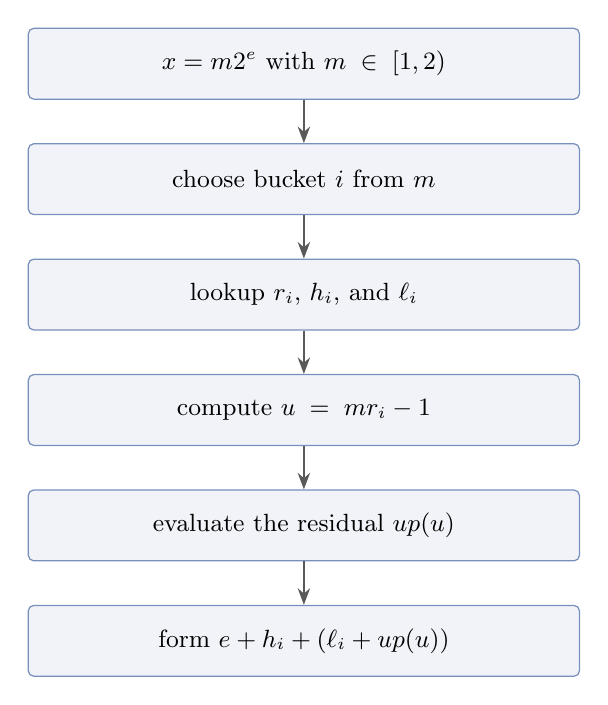
\begin{tikzpicture}[node distance=0.55cm]
    \node (input)  [flowbox] {$x = m2^e$ with $m \;\in\; [1, 2)$};
    \node (bucket) [flowbox, below=of input]  {choose bucket $i$ from $m$};
    \node (lookup) [flowbox, below=of bucket] {lookup $r_i$, $h_i$, and $\ell_i$};
    \node (compu)  [flowbox, below=of lookup] {compute $u \;=\; mr_i - 1$};
    \node (eval)   [flowbox, below=of compu]  {evaluate the residual $up(u)$};
    \node (form)   [flowbox, below=of eval]   {form $e + h_i + (\ell_i + up(u))$};

    \draw[arrow] (input)  -- (bucket);
    \draw[arrow] (bucket) -- (lookup);
    \draw[arrow] (lookup) -- (compu);
    \draw[arrow] (compu)  -- (eval);
    \draw[arrow] (eval)   -- (form);
        \end{tikzpicture}
        \caption{Data flow in the small $\log_2$ core.}
        \Description{Visual aid for the concept described in the caption.}
    \end{figure}
    \FloatBarrier

    The coefficient object is produced from the Sollya polynomial. The table
    object is produced by the table-generation script. Production code should
    store those generated values directly in the implementation or in the nearby
    generated constants file.

    \subsection{What must be proved}

    The table core has more obligations than the small sine kernel. The proof
    needs bounds for:

    \begin{enumerate}
        \item table index selection
        \item reciprocal-table rounding
        \item the size of $u$
        \item the polynomial approximation to $\log_2(1 + u)$
        \item the floating-point evaluation of $u\,p(u)$
        \item the split addition $e + h_i + \ell_i$
        \item the final rounding under each supported mode
    \end{enumerate}

    A Gappa proof is a good fit for the straight-line part after the table entry
    has been chosen. MPFR testing should cover bucket boundaries, values where
    $u$ is near its largest magnitude, exact powers of two, subnormals routed
    through the full log path, and every supported rounding mode.

    \subsection{What this example leaves out}

    A complete function still needs:

    \begin{enumerate}
        \item bit decomposition for all finite positive inputs
        \item handling of zero, negative inputs, NaN, and infinities
        \item subnormal normalization
        \item a larger or more carefully designed table
        \item directed rounding checks
        \item an accurate path for hard cases if correct rounding is the target
    \end{enumerate}

    Real kernels use this same shape: reduce with a table, keep the residual
    small, approximate a smooth transformed function, split constants for
    exactness, and prove the operation sequence that is actually compiled.

    \begin{checkpoint}
        Three questions about the table reduction.
        \begin{enumerate}
            \item What does the reciprocal table actually buy?
            \item Why is $-\log_2(r_i)$ stored as a high part and a low part instead
            of one double?
            \item Why does the polynomial approximate $\log_2(1 + u)/u$ rather than
            $\log_2(m)$ on $[1, 2)$ directly?
        \end{enumerate}
    \end{checkpoint}

    \emph{Milestone.}  You can now open a table-driven kernel in any libm
    source tree and name what each constant is for: which value it
    approximates, how it was split, and which later operation its rounding
    was chosen to keep exact.

% -----------------------------------------------------------------------


    \section{The sign, exponent, and significand split}

    For normal finite binary floating-point values, use the decomposition~\cite{ieee,handbook}:
    \[ x = s_x \cdot 2^{e_x} \cdot (1 + m_x) \]

    This decomposition applies to finite nonzero normal binary floating-point
    numbers.

    \begin{itemize}
        \item $s_x$ is the sign, either $+1$ or $-1$
        \item $e_x$ is the unbiased binary exponent
        \item $m_x$ is the fractional part of the significand
        \item $1 + m_x$ is the normalized significand and lies in $[1, 2)$
    \end{itemize}

    The stored bits mirror the algebra directly. Figure~\ref{fig:doublebits}
    shows the 64-bit double layout. The exponent field holds $e_x$ plus a
    bias of 1023 so it can be stored unsigned. The leading 1 of the
    normalized significand is not stored at all, since normal numbers always
    have it. This layout is why the split is cheap: extracting $e_x$ is a
    shift and a mask on the bit pattern, with no arithmetic error anywhere.

    \begin{figure}[tbp]
        \centering
        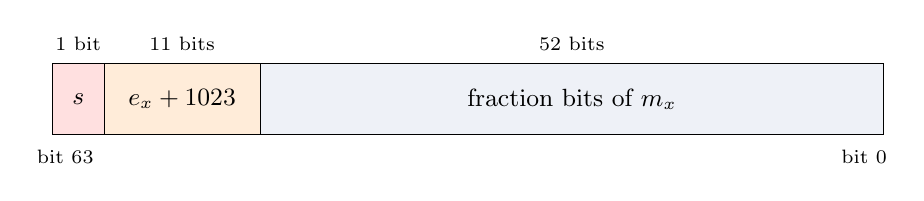
\begin{tikzpicture}[xscale=0.165, yscale=0.9]
    \draw[fill=red!12]    (0,0)  rectangle (4,1);
    \draw[fill=orange!15] (4,0)  rectangle (16,1);
    \draw[fill=figblue!8]   (16,0) rectangle (64,1);
    \node[font=\small] at (2,0.5)  {$s$};
    \node[font=\small] at (10,0.5) {$e_x + 1023$};
    \node[font=\small] at (40,0.5) {fraction bits of $m_x$};
    \node[font=\scriptsize, above] at (2,1.05)  {1 bit};
    \node[font=\scriptsize, above] at (10,1.05) {11 bits};
    \node[font=\scriptsize, above] at (40,1.05) {52 bits};
    \node[font=\scriptsize, below] at (1,-0.08)  {bit 63};
    \node[font=\scriptsize, below] at (62.5,-0.08) {bit 0};
        \end{tikzpicture}
        \caption{The 64-bit double layout, field widths not to scale. The
        exponent is stored with a bias so it is always nonnegative, and the
        leading 1 of the significand is implicit. The algebraic split
            $s_x \cdot 2^{e_x} \cdot (1 + m_x)$ reads straight out of these three
            fields.}
        \label{fig:doublebits}
        \Description{Visual aid for the concept described in the caption.}
    \end{figure}

    Example:
    \[ 6.5 = 1.625 \cdot 2^2 \]
    so:
    \begin{align*}
        s_x &= +1 \\
        e_x &= 2 \\
        m_x &= 0.625 \\
        6.5 &= +1 \cdot 2^2 \cdot (1 + 0.625)
    \end{align*}

    In binary:
    \[ 6.5 = 110.1_2 = 1.101_2 \cdot 2^2 \]

    The exponent carries scale. The significand stays in a fixed interval.
    That turns a many-magnitude problem into a smaller approximation problem plus
    integer exponent bookkeeping.

    The $(1 + m_x)$ form is for normal numbers. Subnormal numbers do not have
    the implicit leading~1 and need normalization or special handling. Zero,
    infinity, and NaN do not fit this decomposition~\cite{ieee}. Negative bases
    for \texttt{pow} need integer-exponent handling before any logarithmic path.

% -----------------------------------------------------------------------


    \section{Argument reduction}

    Approximation works well only on a small interval. Argument reduction is
    how the implementation gets there~\cite{muller,handbook}.

    Start by looking for a part of the function that the format can handle
    directly. Powers of two are cheap because they live in the exponent field.
    Quarter-turns of sine and cosine are cheap because they only change the
    kernel and the sign. The reducer moves that easy part into an integer or a
    small table index, then leaves a residual for the polynomial.

    For \texttt{exp}:
    \[ \exp(x) = 2^k \exp(r) \]
    where:
    \[ k \approx \mathrm{round}\!\left(\frac{x}{\ln(2)}\right) \]
    and:
    \[ r = x - k\ln(2) \]

    The integer $k$ carries the power-of-two scale. The residual $r$ is small
    enough for a short polynomial.

    For \texttt{exp2}, the split is simpler:
    \[ 2^x = 2^k 2^r \]
    where:
    \[ k = \lfloor x \rfloor \]
    and:
    \[ r = x - k \]

    The reconstruction step puts $2^k$ back into the exponent field when the
    result is in range.

    For $\log_2$, the sign, exponent, and significand split gives:
    \[ \log_2(x) = e_x + \log_2(1 + m_x) \]

    For natural logarithm:
    \[ \ln(x) = e_x \ln(2) + \ln(1 + m_x) \]

    The exponent term is exact integer bookkeeping. The hard part is
    approximating the significand term, where $(1 + m_x)$ lies in a fixed
    interval for normal inputs.

    Log implementations therefore usually extract the exponent first, reduce the
    significand, and approximate only a small residual.

    For trig functions, the usual reduction is modulo $\pi/2$ or $\pi/4$,
    followed by quadrant reconstruction.

    Trig reduction is hard for large inputs.  $\pi$ is irrational. If $x$ is
    huge and close to a multiple of $\pi/2$, subtracting $k\pi/2$ can lose the
    useful bits.

    \subsection{Cody-Waite reduction}

    Cody-Waite reduction is the moderate-input reducer. The setup is the same
    as the small \texttt{exp} example: first choose the integer $k$ that removes
    the large scale, then compute the residual. The new problem is that the
    constant being subtracted is not exactly representable, so the constant is
    split before the subtraction starts.

    It represents the reduction constant as a small expansion of machine numbers:
    \[ C = C_\mathrm{hi} + C_\mathrm{mid} + C_\mathrm{lo} \]
    \[ r = x - kC_\mathrm{hi} - kC_\mathrm{mid} - kC_\mathrm{lo} \]

    The split is there to control where rounding first enters the calculation.
    A single rounded constant can already be too crude. For example, reduce
    $x = 30$ for \texttt{exp}. The nearest double to $\ln(2)$ is about
    $9.4 \cdot 10^{-18}$ below the real value. With $k = 43$, the residual
    inherits roughly $4.0 \cdot 10^{-16}$ of constant error before the
    floating-point operations have rounded anything. Around
    $r \approx 0.1947$, that is already about 15~ULPs. The polynomial cannot
    repair bits the reducer never delivered.

    The useful Cody-Waite invariant is exactness. Choose $C_\mathrm{hi}$ with
    enough trailing zero bits that $kC_\mathrm{hi}$ is exactly representable for
    every $k$ produced by the fast reducer. Then arrange the reduction interval
    so $x$ and $kC_\mathrm{hi}$ are close. Sterbenz's lemma makes the first
    subtraction exact, so the leading shared bits cancel without injecting a new
    rounding error. The smaller terms $kC_\mathrm{mid}$ and $kC_\mathrm{lo}$ then
    put back the pieces of $C$ that $C_\mathrm{hi}$ deliberately omitted. Figure~\ref{fig:codywaite}
    shows the bit alignment rather than the arithmetic syntax.

    \begin{figure}[H]
        \centering
        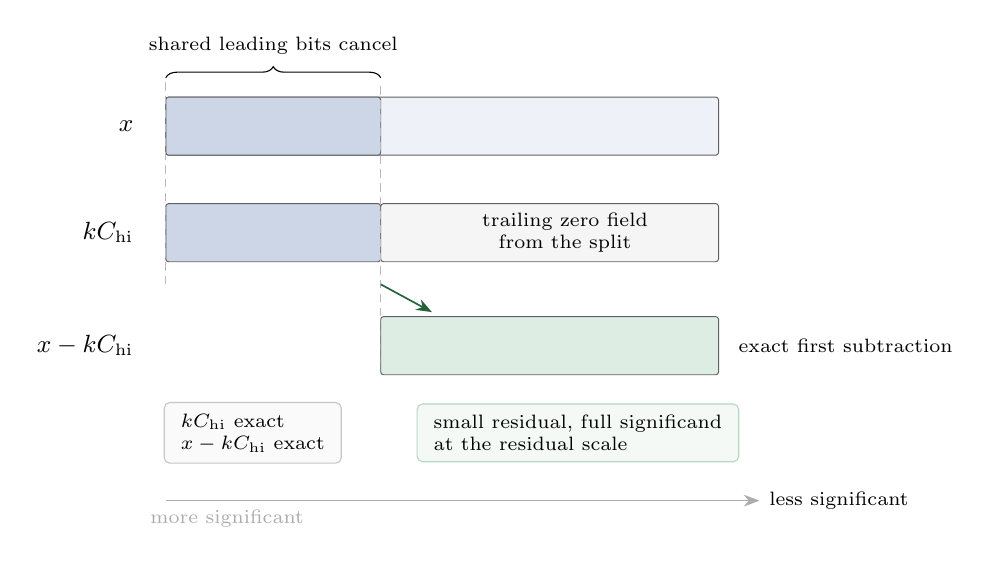
\begin{tikzpicture}[x=0.13cm, y=0.82cm]
            % bit significance axis
            \draw[-{Stealth[length=2mm]}, gray!65] (0,0) -- (58,0)
            node[right, font=\scriptsize, black] {less significant};
            \node[font=\scriptsize, gray!65] at (6,-0.28) {more significant};

            % x row
            \node[bitlabel, left] at (-2.2,5.8) {$x$};
            \draw[bitbar, fill=figblue!8] (0,5.35) rectangle (54,6.25);
            \draw[bitbar, fill=figblue!24] (0,5.35) rectangle (21,6.25);

            % kC_hi row
            \node[bitlabel, left] at (-2.2,4.15) {$kC_\mathrm{hi}$};
            \draw[bitbar, fill=figblue!24] (0,3.7) rectangle (21,4.6);
            \draw[bitbar, fill=gray!8] (21,3.7) rectangle (54,4.6);
            \node[bitnote] at (39,4.15) {trailing zero field\\from the split};

            % cancellation guides
            \draw[densely dashed, gray!55] (0,3.35) -- (0,6.48);
            \draw[densely dashed, gray!55] (21,2.0) -- (21,6.48);
            \draw[decorate, decoration={brace, amplitude=4pt}] (0,6.55) -- (21,6.55)
            node[midway, above=5pt, font=\scriptsize] {shared leading bits cancel};

            % residual row
            \node[bitlabel, left] at (-2.2,2.4) {$x-kC_\mathrm{hi}$};
            \draw[bitbar, fill=figgreen!16] (21,1.95) rectangle (54,2.85);
            \node[bitnote, right] at (55,2.4) {exact first subtraction};
            \draw[-{Stealth[length=2mm]}, figgreen!70!black, semithick]
            (21,3.35) -- (26,2.92);

            % precondition and residual notes
            \node[draw=gray!45, fill=gray!4, rounded corners=2pt,
                inner xsep=6pt, inner ysep=4pt, font=\scriptsize, align=left]
            at (8.5,1.05)
                {$kC_\mathrm{hi}$ exact\\$x-kC_\mathrm{hi}$ exact};
            \node[draw=figgreen!35, fill=figgreen!5, rounded corners=2pt,
                inner xsep=6pt, inner ysep=4pt, font=\scriptsize, align=left,
                anchor=west]
            at (24.5,1.05)
                {small residual, full significand\\at the residual scale};
        \end{tikzpicture}
        \caption{Cody-Waite as a bit-alignment argument. The high split is chosen
        so $kC_\mathrm{hi}$ is exact. When it shares the leading bits of $x$, the
        first subtraction is exact and the residual begins at the lower-significance
        position where the cancellation ended.}
        \label{fig:codywaite}
        \Description{Bit-lane diagram showing that the high split shares leading
        bits with the input, cancels exactly, and leaves a smaller residual.}
    \end{figure}

    Put the exactness conditions in the design note. Each one can fail without an
    obvious local symptom. The integer $k$ must stay inside
    the range used when choosing the trailing zeros of $C_\mathrm{hi}$. The
    values $x$ and $kC_\mathrm{hi}$ must be within a factor of two for
    Sterbenz's lemma to apply~\cite{handbook}. The residual must also stay
    large enough, relative to the discarded $kC_\mathrm{lo}$ tail, that the
    later additions do not erase the bits the split preserved. All of these
    are checkable from the reducer's input range.

    \subsection{Payne-Hanek reduction}

    Payne-Hanek reduction is the large-input reducer for trig functions. It
    answers the same question Cody-Waite answers, namely which multiple of
    $\pi/2$ should be removed and what residual remains. The difference is that
    the subtraction is too delicate to do directly, so the algorithm computes the
    quadrant first from a high-precision reciprocal of $\pi/2$.

    It uses a long table of the reduction constant and a fixed-precision integer
    multiply~\cite{muller}.

    Ordinary double arithmetic is not strong enough to reduce every binary64 value
    modulo $\pi/2$. Some inputs land extraordinarily close to a nonzero multiple
    of $\pi/2$. A direct subtraction then has to cancel sixty or more leading bits
    and still leave a trustworthy residual. That is outside the useful range of a
    short Cody-Waite split.

    The Payne-Hanek route computes the fractional part of
    $x \cdot \tfrac{2}{\pi}$ instead of subtracting $k\pi/2$ directly~\cite{payne1983}.
    The table stores $2/\pi$ as integer words, with comfortably more than a
    thousand bits for a binary64 implementation. Since $x$ is a significand times
    a power of two, its exponent selects the only window of table words that can
    influence the quadrant and the high bits of the residual. Words above that
    window contribute only discarded multiples of~4. Words below it cannot reach
    the rounding decision.

    The core operation is an integer product: the 53-bit significand of $x$ times
    the selected table window. The two bits around the binary point give
    $k \bmod 4$. The remaining fractional part is converted back to floating point
    and multiplied by $\pi/2$ to form the reduced argument. Guard bits in the
    window are sized from the worst possible cancellation. For binary64, that
    worst case is known by exhaustive search over the exponent range, which fixes
    the required window once rather than by guesswork~\cite{muller}.

    \begin{figure}[tbp]
        \centering
        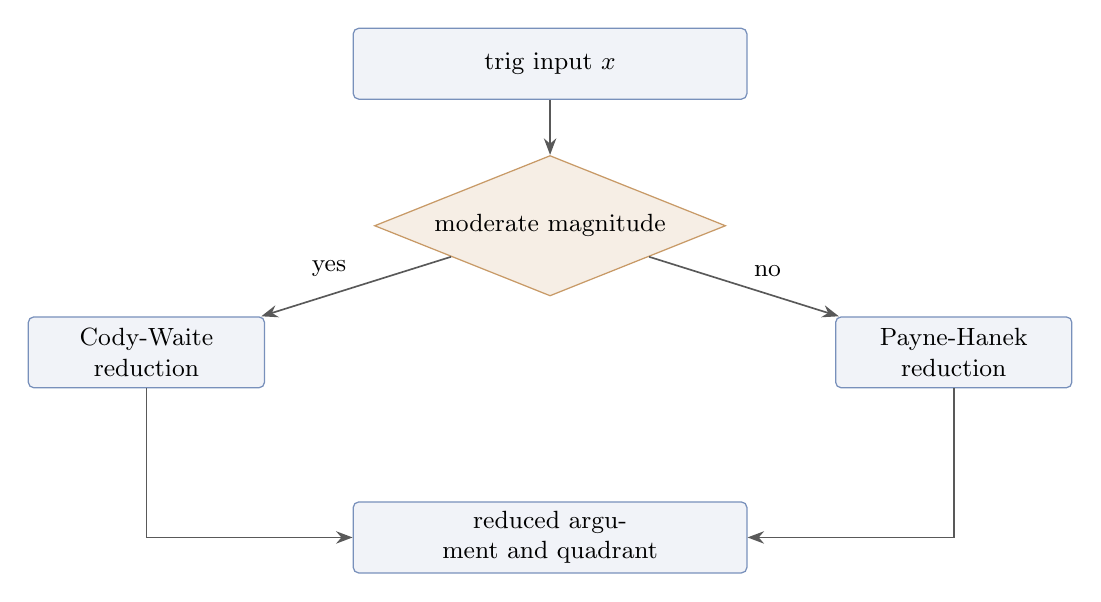
\begin{tikzpicture}[node distance=0.7cm and 2.5cm]
    \node (inp)  [flowbox, minimum width=5cm] {trig input $x$};
    \node (dec)  [decisionbox, below=of inp]      {moderate magnitude};
    \node (cw)   [flowbox, minimum width=3cm, below left=of dec]  {Cody-Waite\\reduction};
    \node (ph)   [flowbox, minimum width=3cm, below right=of dec] {Payne-Hanek\\reduction};
    \node (out)  [flowbox, minimum width=5cm, below=2.6cm of dec] {reduced argu-\\ment and quadrant};

    \draw[arrow] (inp) -- (dec);
    \draw[arrow] (dec) -- node[above left,  font=\small]{yes} (cw);
    \draw[arrow] (dec) -- node[above right, font=\small]{no}  (ph);
    \draw[arrow] (cw)  |- (out);
    \draw[arrow] (ph)  |- (out);
        \end{tikzpicture}
        \caption{Typical trig reduction split between moderate and large inputs.}
        \Description{Visual aid for the concept described in the caption.}
    \end{figure}

    \subsection{Trig quadrant reconstruction}

    \[ x = k\frac{\pi}{2} + r \]

    The reducer returns an integer $k$ and a small residual $r$. The value of
    $k \bmod 4$ decides which small kernel reconstructs the result~\cite{muller}.

    \begin{table}[tbp]
        \centering
        \begin{tabular}{cl}
            \toprule
            $k \bmod 4$ & $\sin(x)$ reconstruction \\
            \midrule
            0           & $\sin(r)$                \\
            1           & $\cos(r)$                \\
            2           & $-\sin(r)$               \\
            3           & $-\cos(r)$               \\
            \bottomrule
        \end{tabular}
    \end{table}

    Figure~\ref{fig:quadrants} shows where the table comes from. Reducing
    modulo $\pi/2$ lands the angle in one of four quadrants of the unit
    circle. In each quadrant, the sine of the full angle equals plus or
    minus the sine or cosine of the small residual, so two kernels and a sign
    cover the whole circle.

    \begin{figure}[tbp]
        \centering
        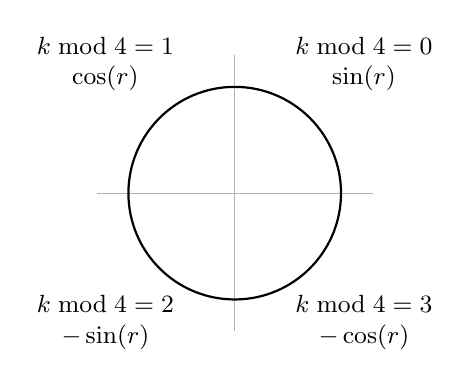
\begin{tikzpicture}[scale=1.35]
    \draw[gray!60] (-1.3,0) -- (1.3,0);
    \draw[gray!60] (0,-1.3) -- (0,1.3);
    \draw[thick] (0,0) circle (1);
    \node[font=\small, align=center] at (45:1.72)
        {$k \bmod 4 = 0$\\$\sin(r)$};
    \node[font=\small, align=center] at (135:1.72)
        {$k \bmod 4 = 1$\\$\cos(r)$};
    \node[font=\small, align=center] at (225:1.72)
        {$k \bmod 4 = 2$\\$-\sin(r)$};
    \node[font=\small, align=center] at (315:1.72)
        {$k \bmod 4 = 3$\\$-\cos(r)$};
        \end{tikzpicture}
        \caption{Quadrant reconstruction for $\sin(x)$. The reducer writes
            $x = k\pi/2 + r$, the quadrant index $k \bmod 4$ picks the kernel and
            the sign, and the polynomial only ever evaluates near zero.}
        \label{fig:quadrants}
        \Description{Visual aid for the concept described in the caption.}
    \end{figure}

    A full trig function is therefore more than one polynomial. The reducer and
    quadrant logic choose the kernel and the returned sign.

    \subsection{Reduction error}

    Reduction has its own error.

    If the polynomial was proved for an exact reduced argument $r$, but the
    implementation computes $r$ with too much error, the proof no longer applies.

    Decide the total error target first. Give part of that budget to reduction.
    The reducer should carry enough extra precision that its error stays below
    that budget.

    For many functions, this means split constants or a double-word reduced
    argument. For very large trig inputs, it can mean a separate large-argument
    reducer.

    \begin{checkpoint}
        This one is a pencil-and-paper exercise. Reduce $x = 1000$ for
        \texttt{exp} using one rounded constant $L$ for $\ln(2)$. Compute $k$,
        then the drift $k(\ln 2 - L)$, then express the drift in ULPs of the
        residual. The numbers from Section~\ref{sec:relabs} and the worked
        $x = 30$ case above contain everything needed.
    \end{checkpoint}

% -----------------------------------------------------------------------


    \section{Evaluating the polynomial}

    After Sollya gives coefficients, the implementation still has to evaluate
    the polynomial in floating point.

    The mathematical polynomial and the C++ expression are different objects.
    Sollya bounds the exact polynomial. The compiler runs a particular sequence
    of additions, multiplications, and FMA operations, and every one of those
    operations can round. Pick the evaluation shape before writing the Gappa goal,
    because changing the shape changes the proof.

    \subsection{Horner evaluation}

    Horner evaluation is the usual default:
    \[ p(x) = c_0 + x(c_1 + x(c_2 + x(\cdots))) \]

    It uses few operations and maps well to FMA~\cite{muller,handbook}.

    With FMA, one step can be:
    \begin{lstlisting}[style=cpp]
r = fma(r, x, c);
    \end{lstlisting}

    That rounds the multiply-add once.

    \texttt{std::fma} comes with caveats. Unless the build pins
    \texttt{FP\_CONTRACT} or the equivalent flag, a compiler may fuse a
    written \texttt{a*b + c} on its own, or decline to, so write
    \texttt{std::fma} where the proof needs one rounding and separate
    operations where it needs two. On targets without an FMA instruction
    the call is emulated in software, still correctly rounded but far
    slower, so check the target before designing a kernel around dozens of
    them. And \texttt{std::fma} is usable in constant expressions only
    from C++23, while compile-time arithmetic always rounds to nearest, so
    a constexpr kernel can legitimately produce different bits than the
    same kernel running under a directed mode.

    \subsection{Estrin evaluation}

    Estrin evaluation groups terms so more work can happen in
    parallel~\cite{handbook}.

    Example:
    \[ c_0 + c_1 x + c_2 x^2 + c_3 x^3 \]
    can be grouped as:
    \[ (c_0 + c_1 x) + x^2(c_2 + c_3 x) \]

    This can be faster on wide cores. It can also need more temporaries. Use it
    when measurements show that it helps.


    \begin{checkpoint}
        Mini exercise: choose an evaluation shape. For a degree-7 polynomial,
        compare plain Horner with an Estrin-style grouping.
        \begin{enumerate}
            \item Which one has the shorter dependency chain?
            \item Which one is simpler to prove operation-for-operation?
            \item If a target has slow FMA but good instruction-level parallelism,
            which one would you benchmark first?
        \end{enumerate}
    \end{checkpoint}

    \subsection{Double-word evaluation}

    Some kernels need more precision in part of the evaluation.

    Common tools include Fast2Sum, 2Sum, 2MultFMA, Veltkamp-Dekker splitting,
    double-double arithmetic, and compensated Horner evaluation~\cite{muller,handbook}.

    The common trick is to represent one value as an unevaluated sum of two
    doubles. The high part carries the leading 53 bits, the low part carries
    the next 53, and the pair behaves like a number with roughly 106
    significand bits as long as every operation tracks both pieces.
    Figure~\ref{fig:doubleword} shows the layout. The error terms that
    Fast2Sum and 2MultFMA recover are exactly the low parts this
    representation needs.

    \begin{figure}[tbp]
        \centering
        \begin{tikzpicture}[xscale=0.165, yscale=0.85]
    \draw[fill=figblue!10]  (0,0)  rectangle (26.5,1);
    \draw[fill=green!15] (28,0) rectangle (54.5,1);
    \node[font=\small] at (13.25,0.5) {hi: leading 53 bits};
    \node[font=\small] at (41.25,0.5) {lo: next 53 bits};
    \draw[decorate, decoration={brace, amplitude=5pt}] (0,1.25) -- (54.5,1.25)
    node[midway, above=6pt, font=\small] {value $=$ hi $+$ lo};
    \node[font=\scriptsize, below] at (27.25,-0.15)
        {$|\mathrm{lo}| \le \tfrac{1}{2}\,\mathrm{ulp}(\mathrm{hi})$, so the
    parts do not overlap};
        \end{tikzpicture}
        \caption{A double-word value. Two ordinary doubles, kept as an
        unevaluated sum, act as one number with about twice the significand
        bits. No new hardware type is involved, only bookkeeping.}
        \label{fig:doubleword}
        \Description{Visual aid for the concept described in the caption.}
    \end{figure}

    Do not use double-double everywhere by default. Use it where the error
    budget needs it.

    The most useful extra precision is usually local. It protects one reduction,
    one product, or one reconstruction step. Treat it as a tool for a specific
    bound, not as a blanket fix.

% -----------------------------------------------------------------------


    \section{Fast precision and accurate precision}

    Many elementary functions use more than one precision tier.

    The reason is not that every input needs wide arithmetic. Most inputs land far
    from a rounding boundary, so a cheaper computation already proves the final
    rounded result. A small fraction of inputs land too close to decide cheaply.
    Those inputs are rerun with a wider, slower path.

    Keep the fast path cheap. It handles ordinary inputs where a modest amount of
    extra precision is enough. The accurate path handles cases where
    the result is too close to a rounding boundary\footnote{A rounding boundary is the point where the selected floating-point result changes. Under round-to-nearest, it is usually the midpoint between two adjacent representable values.}, or where the fast path cannot
    prove the final rounding decision.

    For float functions, the implementation can often use double or double-double
    arithmetic for the fast path. Some cases may need a wider accurate path.

    For double functions, the fast path usually needs a double-double-like
    computation. That does not mean every operation should behave like a complete
    higher-precision type. A full double-double type that renormalizes after
    every operation is often too expensive for the hot path.

    A faster pattern is to arrange the computation so that important intermediate
    pieces are exact, or have a known error, and normalize only where the bound
    needs it. This is less general than a full double-double type, but it fits a
    fixed numerical kernel better.

    The accurate path may use a dyadic\footnote{A dyadic number is a rational number whose denominator is a power of two. A fixed-precision dyadic format is useful in proofs because its arithmetic tracks binary floating-point structure without using a hardware type directly.} floating-point type with a fixed integer
    significand, such as a 128-bit or 256-bit dyadic format. This gives a large
    exponent range and controlled precision without relying on hardware quad
    precision.

    Quad precision and double-double are not interchangeable.

    Quad precision has a much larger exponent range than double-double. A pair
    of doubles gives extra significand bits, but it does not cheaply give the
    exponent range of a true quad format. A dyadic format can be a better
    accurate-path type when the algorithm needs wide range and predictable fixed
    precision.

    One tiering pattern is:

    \begin{table}[tbp]
        \centering
        \begin{tabular}{ll}
            \toprule
            Tier                         & Role                       \\
            \midrule
            double or double-double-like & Fast path                  \\
            128-bit dyadic               & First accurate path        \\
            256-bit dyadic               & Hard-case path when needed \\
            \bottomrule
        \end{tabular}
    \end{table}

    This is especially relevant for \texttt{pow}. A double \texttt{pow}
    implementation is harder than a float \texttt{pow} implementation because the
    final result has a 53-bit significand. The intermediate log, multiply, and
    exp reconstruction must leave enough margin for correct rounding.

% -----------------------------------------------------------------------


    \section{Lookup tables}

    Lookup tables in elementary functions are not only cached constants.

    A useful table usually comes from a small algebraic target. Split the input
    interval into buckets, choose one number per bucket that makes the residual
    small, and store the correction needed to make the identity true again. The
    polynomial then sees the residual, not the original input.

    A table entry usually exists to make one reduction step cheaper, more
    accurate, or both. For log and pow, common table values include
    approximations to quantities like $-\log_2(r)$, split into pieces.

    A split table might store:
    \[ a = -\log_2(r) \]
    and:
    \[ a = a_\mathrm{hi} + a_\mathrm{mid} + a_\mathrm{lo} \]

    Choose the split for a reason. A high part may be rounded to a smaller
    precision so that a later multiplication is exact, or so that adding it to an
    exponent does not lose important bits.

    Table generation should start from an invariant, not from a literal list of
    constants.

    A table-generation note should record:

    \begin{enumerate}
        \item how the index is chosen
        \item what real value each entry approximates
        \item how the entry is split
        \item which later operation is meant to be exact or tightly bounded
        \item what interval remains after the table reduction
        \item which precision tier uses the table
    \end{enumerate}

    For \texttt{powf}, the fast path may use tables split into double-double or
    triple-double pieces because the target result is float. For \texttt{pow} in
    double, the accurate paths may need tables generated directly for the wider
    dyadic type used in that path.

    Do not assume one table layout fits every precision tier.

    If the accurate pass uses a 128-bit dyadic format, generate a table suited to
    that format. If there is a 256-bit hard-case path, generate the table for
    that path as well. The values may represent the same mathematical constants,
    but the split, precision, and exactness constraints can be different.

    Without its generation rule, a table is hard to audit. With the invariant
    recorded, it is part of the proof.

    \subsection{Log table reduction}

    \[ \log_2(1 + m_x) = -\log_2(r_i) + \log_2(r_i(1 + m_x)) \]

    Define:
    \[ u = r_i(1 + m_x) - 1 \]

    Then:
    \[ \log_2(1 + m_x) = -\log_2(r_i) + \log_2(1 + u) \]

    The table value $r_i$ is chosen so that $u$ is small. Usually $r_i$ is close
    to the reciprocal of a representative value in the bucket. Then
    $r_i(1 + m_x)$ lands near 1, so $u = r_i(1 + m_x) - 1$ lands near 0. The
    polynomial only approximates $\log_2(1 + u)$ on that smaller interval. The
    table entry supplies the correction term $-\log_2(r_i)$.

    That is the value of the table. It does more than avoid a computation. It
    makes the residual small enough for a cheaper and more accurate polynomial.
    Section~\ref{sec:log2} uses the same pattern with bucket reciprocals and
    split $-\log_2(r_i)$ constants.

% -----------------------------------------------------------------------


    \section{Why pow is harder than exp or log}

    \texttt{pow} combines the difficulties of log and exp.

    Start with the easy case: positive finite $x$ and a finite $y$. In that case,
    the identity is a composition of two one-argument functions. The production
    function cannot stop there, because negative bases, zeros, infinities, NaNs,
    and integer exponents all have separate rules, but the positive finite path
    explains why the core is expensive.

    For positive finite $x$, the usual shape is:
    \begin{align*}
        \mathrm{pow}(x, y) &= \exp(y \log(x)) \\
        \mathrm{pow}(x, y) &= 2^{y \log_2(x)}
    \end{align*}

    \[ y \log_2(x) = y(e_x + \log_2(1 + m_x)) \]

    That is why pow implementations often contain a log core, table reduction for
    the significand, split constants, and extra precision around the product
    $y \log_2(x)$. A small error in the log value can be magnified by $y$, then
    carried into the exp reconstruction. Figure~\ref{fig:powcompose} shows
    the chain.

    \begin{figure}[tbp]
        \centering
        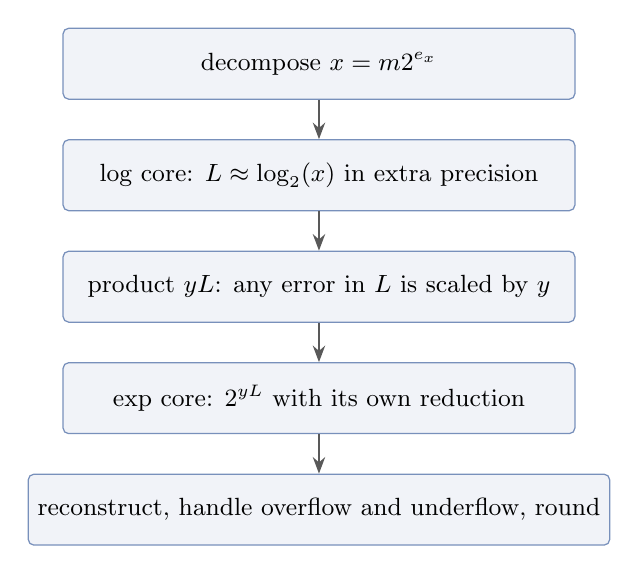
\begin{tikzpicture}[node distance=0.5cm]
    \node (dec) [flowbox, minimum width=6.5cm] {decompose $x = m2^{e_x}$};
    \node (log) [flowbox, below=of dec, minimum width=6.5cm]
    {log core: $L \approx \log_2(x)$ in extra precision};
    \node (mul) [flowbox, below=of log, minimum width=6.5cm]
    {product $yL$: any error in $L$ is scaled by $y$};
    \node (exp) [flowbox, below=of mul, minimum width=6.5cm]
    {exp core: $2^{yL}$ with its own reduction};
    \node (rnd) [flowbox, below=of exp, minimum width=6.5cm]
    {reconstruct, handle overflow and underflow, round};

    \draw[arrow] (dec) -- (log);
    \draw[arrow] (log) -- (mul);
    \draw[arrow] (mul) -- (exp);
    \draw[arrow] (exp) -- (rnd);
        \end{tikzpicture}
        \caption{pow as a composition. Each core is a full reduction,
            approximation, and reconstruction pipeline of its own, and the product
            in the middle amplifies whatever error the log core left behind.}
        \label{fig:powcompose}
        \Description{Visual aid for the concept described in the caption.}
    \end{figure}

    That hides several problems.

    First, $\log(x)$ needs its own range reduction, tables, approximation, and
    reconstruction.

    Second, $y \log(x)$ can magnify error. The relative error of the final
    result is roughly $\ln(2)$ times the absolute error of the product
    $y \log_2(x)$, so landing within $2^{-60}$ of the true result means
    knowing that product to about $2^{-60}$ absolutely. When $y$ is as
    large as $2^{10}$, the log core must deliver $\log_2(x)$ to about
    $2^{-70}$, seventeen bits past what a plain double can carry. This is
    why pow cores keep the log in double-double or wider from the start.

    Third, \texttt{exp} has to reconstruct the final result, including overflow
    and underflow behavior.

    Fourth, \texttt{pow} has many special cases. The C++ contract pins a
    long list of them exactly, and several are easy to guess wrong:

    \begin{table}[tbp]
        \centering
        \begin{tabular}{ll}
            \toprule
            Input                                                 & Required result                \\
            \midrule
            $\mathrm{pow}(x, \pm 0)$                              & 1 for every $x$, including NaN \\
            $\mathrm{pow}(1, y)$                                  & 1 for every $y$, including NaN \\
            $\mathrm{pow}(-1, \pm\infty)$                         & 1                              \\
            $\mathrm{pow}(\pm 0, y)$, $y$ a negative odd integer  & $\pm\infty$, divide-by-zero    \\
            $\mathrm{pow}(\pm 0, y)$, $y$ a positive odd integer  & $\pm 0$                        \\
            $\mathrm{pow}(x, y)$, finite $x < 0$, non-integer $y$ & NaN, invalid                   \\
            $\mathrm{pow}(x, -\infty)$, $|x| < 1$                 & $+\infty$                      \\
            $\mathrm{pow}(x, +\infty)$, $|x| < 1$                 & $+0$                           \\
            \bottomrule
        \end{tabular}
    \end{table}

    The table is abridged. The full list lives in Annex~F of the C standard
    and transfers to C++ through \texttt{<cmath>}. Exact and near-exact
    cases also need dedicated paths: integer exponents of moderate size,
    bases that are powers of two, and $y = 0.5$, which agrees with
    \texttt{sqrt} everywhere except that $\mathrm{pow}(-0, 0.5)$ returns
    $+0$ while $\mathrm{sqrt}(-0)$ returns $-0$.


    \begin{checkpoint}
        Mini exercise: route four \texttt{pow} calls before the polynomial path.
        For each call, say whether it can use the positive finite core, an integer
        exponent path, or a special-case return.
        \begin{enumerate}
            \item $\mathrm{pow}(2, 10)$
            \item $\mathrm{pow}(-2, 3)$
            \item $\mathrm{pow}(-2, 0.5)$
            \item $\mathrm{pow}(1, \mathrm{NaN})$
        \end{enumerate}
    \end{checkpoint}

    Correct rounding compounds all of it. Double-precision \texttt{pow}
    stayed out of reach for production libraries far longer than \texttt{exp}
    or \texttt{log}, and the CORE-MATH project documents both the algorithms
    and the remaining worst-case questions involved~\cite{coremathpaper}.

    Because of this, \texttt{pow} is not a good first elementary function.

    A better path is:

    \begin{enumerate}
        \item implement one exp-family function
        \item implement one log-family function
        \item learn the reduction, table, polynomial, and rounding structure
        \item then implement pow
    \end{enumerate}

    \texttt{pow} is best understood as a composition of those two families, plus
    a large special-case layer and a harder final-rounding problem.

% -----------------------------------------------------------------------


    \section{Compiler behavior}
    \label{sec:compiler}

    An error proof assumes a specific sequence of floating-point operations. The
    compiler may change that sequence unless the source and build settings prevent
    it.

    The main hazards are worth naming explicitly:

    \begin{table}[H]
        \centering
        \begin{tabular}{ll}
            \toprule
            Hazard                            & Why it matters                                  \\
            \midrule
            FMA contraction                   & \texttt{a*b + c} may become one fused operation \\
            Reassociation                     & fast-math may reorder arithmetic                \\
            Default rounding assumptions      & directed modes may be ignored                   \\
            Hidden precision                  & intermediates may have different width          \\
            Floating-point environment access & \texttt{fenv} support differs by compiler       \\
            \bottomrule
        \end{tabular}
    \end{table}

    These two expressions do not have the same rounding behavior:
    \begin{lstlisting}[style=cpp]
a * b + c
    \end{lstlisting}
    \begin{lstlisting}[style=cpp]
std::fma(a, b, c)
    \end{lstlisting}

    The first can round the product and then the sum. The second rounds once.

    \begin{pitfall}{proving one program and compiling another}
        If a proof needs FMA, use FMA explicitly. If a proof needs the live
        rounding mode, compile in a mode that respects it. Do not prove one
        operation sequence and compile a different one~\cite{handbook}.
        Fast-math flags break the bounds in this guide.
    \end{pitfall}

    This also affects double-double arithmetic. Some exact multiplication
    algorithms for double-double arithmetic without FMA are only valid under
    round-to-nearest. Making them correct under directed rounding can require
    extra handling. That cost belongs in the design.

    \subsection{The flags that matter}

    The hazards above map onto a small set of compiler switches. GCC and
    Clang spellings are shown. MSVC bundles roughly the same choices into
    \texttt{/fp:fast}, \texttt{/fp:precise}, and \texttt{/fp:strict}.

    \begin{table}[H]
        \centering
        \begin{tabular}{lp{8cm}}
            \toprule
            Flag & Effect on a math kernel \\
            \midrule
            \texttt{-ffast-math}
            & Bundle of promises: reassociation, no signed zeros, no NaN or
            infinity handling, reciprocal shortcuts, and on some targets
            flushing subnormals to zero. Any one of them invalidates an
            IEEE-based proof. Defines \texttt{\_\_FAST\_MATH\_\_}, which a
            header can detect and warn on. \\
            \texttt{-ffp-contract=fast}
            & Lets the compiler fuse \texttt{a*b + c} even outside fast math.
            It is the default on some compiler and target combinations, so
            pin it rather than assume it. \\
            \texttt{-fno-math-errno}
            & Stops libm calls from maintaining \texttt{errno}. The C
            contract allows error reporting through \texttt{errno}, through
            floating-point flags, or both, advertised by
            \texttt{math\_errhandling}. Maintaining \texttt{errno} blocks
            vectorization and inlining, which is why many libraries document
            that they never set it. \\
            \texttt{-frounding-math}
            & Tells the compiler not to assume round to nearest, which
            disables constant folding and code motion that would break
            \texttt{fesetround} callers. \\
            \texttt{-fexcess-precision=standard}
            & On targets that evaluate in wider registers, x87 being the
            classic case, forces predictable rounding of intermediates.
            \texttt{FLT\_EVAL\_METHOD} reports the policy. Double rounding
            through a wider format can change results, so platforms where it
            is nonzero need their own validation pass. \\
            \bottomrule
        \end{tabular}
    \end{table}
    \FloatBarrier

    For library work, keep the policy simple: build with precise semantics, state
    the flags next to every measured number, and treat a user who links the kernel
    into a fast-math build as outside the proof.

    \FloatBarrier

% -----------------------------------------------------------------------


    \section{The error budget}

    \[
        E_\mathrm{total} \le E_\mathrm{reduce} + E_\mathrm{approx} +
        E_\mathrm{eval} + E_\mathrm{reconstruct} + E_\mathrm{round}
    \]

    \begin{itemize}
        \item $E_\mathrm{reduce}$ comes from argument reduction
        \item $E_\mathrm{approx}$ comes from replacing the function with a
        polynomial or rational function
        \item $E_\mathrm{eval}$ comes from evaluating that approximation in
        floating point
        \item $E_\mathrm{reconstruct}$ comes from scaling, sign changes, table
        corrections, and final algebra
        \item $E_\mathrm{round}$ is the margin needed for the final rounding
        decision
    \end{itemize}

    Use this inequality as a model for thinking about the implementation. It is
    not always the final tight proof. It prevents a common mistake: proving the
    polynomial and forgetting the rest of the function.

    A small worked allocation makes the model concrete. Suppose a double
    function targets faithful rounding, so everything before the final
    rounding must stay below half an ULP. Within the binade $[1, 2)$ that is
    at worst $2^{-54}$ in relative terms. One workable split:

    \begin{table}[tbp]
        \centering
        \begin{tabular}{lll}
            \toprule
            Term                     & Bound              & Share of $2^{-54}$ \\
            \midrule
            $E_\mathrm{reduce}$      & $2^{-60}$          & about 2\%          \\
            $E_\mathrm{approx}$      & $2^{-58}$          & about 6\%          \\
            $E_\mathrm{eval}$        & $2^{-57}$          & about 12\%         \\
            $E_\mathrm{reconstruct}$ & $2^{-59}$          & about 3\%          \\
            \midrule
            total                    & $15 \cdot 2^{-60}$ & under a quarter    \\
            \bottomrule
        \end{tabular}
    \end{table}

    These numbers are illustrative rather than prescriptive. What matters is
    the shape of the allocation. Each stage gets an explicit slice, the
    slices sum with margin to spare, and a stage that cannot meet its slice
    forces a redesign before any code is written.

% -----------------------------------------------------------------------


    \section{Rounding modes}
    \label{sec:roundingmodes}

    Every floating-point operation ends with the same step. The arithmetic
    produces a value that is usually not representable, and a rule picks which
    representable neighbor to return. IEEE~754 defines four such rules for
    binary formats, and C++ exposes them through \texttt{<cfenv>}~\cite{ieee}.

    This matters because the polynomial proof is not finished until the final
    result is rounded according to the active rule. A value that is safe under
    round to nearest may be one ULP wrong under upward rounding if the proof only
    bounded the nearest-neighbor case.

    \begin{table}[tbp]
        \centering
        \begin{tabular}{lll}
            \toprule
            Mode                           & C++ \texttt{fenv} constant & Guarantee                    \\
            \midrule
            Round to nearest, ties to even & \texttt{FE\_TONEAREST}     & closest neighbor             \\
            Round toward positive infinity & \texttt{FE\_UPWARD}        & never below the exact result \\
            Round toward negative infinity & \texttt{FE\_DOWNWARD}      & never above the exact result \\
            Round toward zero              & \texttt{FE\_TOWARDZERO}    & magnitude never grows        \\
            \bottomrule
        \end{tabular}
    \end{table}

    Round to nearest is the default on every mainstream platform and the only
    mode most code ever runs in. When the exact result lands exactly halfway
    between two neighbors, the tie goes to the neighbor whose last
    significand bit is zero. The tie rule earns its keep in long
    computations: always rounding ties upward would push results steadily in
    one direction, while ties to even alternates the direction and the bias
    cancels on average~\cite{handbook}.

    The three directed modes trade closeness for a guaranteed direction. That
    guarantee is what interval arithmetic\footnote{Interval arithmetic tracks a lower and upper bound for each value instead of one approximate value. With directed rounding, the exact result can be kept inside the interval.} buys: run a computation
    once rounding down and once rounding up, and the true result is bracketed
    between the two outputs. Directed modes also appear in validated
    numerics and in tests that hunt for rounding sensitivity.
    Figure~\ref{fig:roundingmodes} shows all four decisions on one input and
    its negation.

    \begin{figure}[tbp]
        \centering
        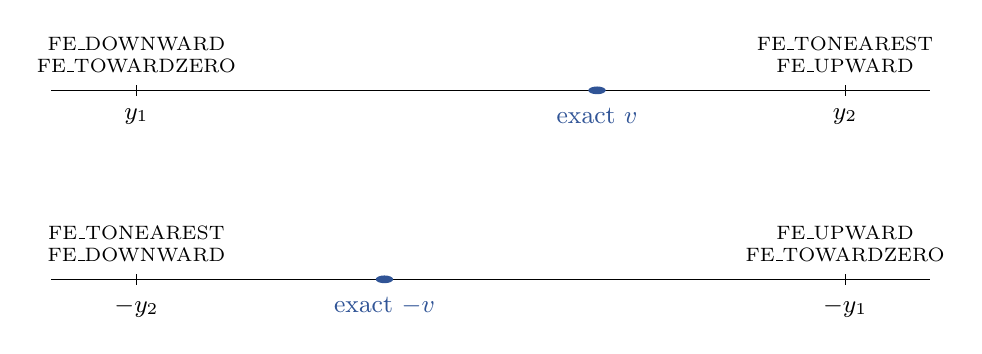
\begin{tikzpicture}[xscale=9]
            % positive value
            \draw (-0.12,0) -- (1.12,0);
            \draw (0,-0.07) -- (0,0.07);
            \draw (1,-0.07) -- (1,0.07);
            \node[below=3pt, font=\small] at (0,0) {$y_1$};
            \node[below=3pt, font=\small] at (1,0) {$y_2$};
            \fill[figblue] (0.65,0) circle (0.35pt and 1.4pt);
            \node[below=3pt, font=\small, figblue] at (0.65,0) {exact $v$};
            \node[above=3pt,  font=\scriptsize, align=center] at (0,0)
                {FE\_DOWNWARD\\FE\_TOWARDZERO};
            \node[above=3pt,  font=\scriptsize, align=center] at (1,0)
                {FE\_TONEAREST\\FE\_UPWARD};

            % negated value
            \begin{scope}[yshift=-2.4cm]
                \draw (-0.12,0) -- (1.12,0);
                \draw (0,-0.07) -- (0,0.07);
                \draw (1,-0.07) -- (1,0.07);
                \node[below=3pt, font=\small] at (0,0) {$-y_2$};
                \node[below=3pt, font=\small] at (1,0) {$-y_1$};
                \fill[figblue] (0.35,0) circle (0.35pt and 1.4pt);
                \node[below=3pt, font=\small, figblue] at (0.35,0) {exact $-v$};
                \node[above=3pt, font=\scriptsize, align=center] at (0,0)
                    {FE\_TONEAREST\\FE\_DOWNWARD};
                \node[above=3pt, font=\scriptsize, align=center] at (1,0)
                    {FE\_UPWARD\\FE\_TOWARDZERO};
            \end{scope}
        \end{tikzpicture}
        \caption{What each mode returns when the exact result $v$ falls between
        the representable neighbors $y_1 < y_2$, shown for $v$ and for $-v$.
        Round to nearest ignores the sign. The directed modes do not: round
        toward zero picks the lower neighbor for positive values and the upper
        neighbor for negative ones.}
        \label{fig:roundingmodes}
        \Description{Visual aid for the concept described in the caption.}
    \end{figure}

    \subsection{The C++ mechanics}

    Rounding mode is dynamic state, not a property of the source code.
    \texttt{std::fesetround} changes it for the calling thread,
    \texttt{std::fegetround} reads it, and any function may be called under
    whatever mode the caller installed. Three consequences matter for
    library work.

    First, a function does not get to choose the mode it runs under. If the
    caller installed \texttt{FE\_UPWARD}, every add, multiply, and FMA inside
    the function rounds upward, whether the author planned for that or not.

    Second, compile-time arithmetic ignores the dynamic mode. Constant
    folding and \texttt{constexpr} evaluation round to nearest. The same
    expression can therefore produce different bits at compile time and at
    run time, and a cached compile-time constant can disagree with the
    runtime computation that recreates it.

    Third, the optimizer assumes the default mode unless told otherwise. The
    \texttt{\#pragma STDC FENV\_ACCESS} switch exists for this, but support
    is uneven across compilers, so code that mixes \texttt{fesetround} with
    ordinary arithmetic needs testing on every toolchain it claims to
    support.

    The effect is easy to reproduce. The program
    \path{docs/approximating_functions/cpp/directed_rounding_demo.cpp}
    evaluates two expressions under each mode, compiled with
    \texttt{-frounding-math} so the compiler does not fold them:
    \begin{lstlisting}[style=shell]
c++ -std=c++17 -O2 -frounding-math \
    docs/approximating_functions/cpp/directed_rounding_demo.cpp \
    -o directed_rounding_demo && ./directed_rounding_demo
    \end{lstlisting}

    \begin{lstlisting}[style=output]
FE_TONEAREST   1/3 = 0x1.5555555555555p-2   0.1+0.1+0.1 = 0x1.3333333333334p-2
FE_UPWARD      1/3 = 0x1.5555555555556p-2   0.1+0.1+0.1 = 0x1.3333333333334p-2
FE_DOWNWARD    1/3 = 0x1.5555555555555p-2   0.1+0.1+0.1 = 0x1.3333333333333p-2
FE_TOWARDZERO  1/3 = 0x1.5555555555555p-2   0.1+0.1+0.1 = 0x1.3333333333333p-2
    \end{lstlisting}

    The quotient moves by one bit under \texttt{FE\_UPWARD} and the repeated
    sum moves under the two downward modes. The source is identical in every
    row, only the installed mode differs, and a library function has to be
    correct under all four.

    \subsection{Why round-to-nearest proofs do not transfer}

    A bound proved under round to nearest does not automatically hold in the
    directed modes.

    The most direct problem is the unit rounding error, which doubles. One
    operation is off by at most half an ULP under round to nearest, but by up
    to a full ULP under a directed mode, so every term of an error budget
    grows.

    A subtler problem is that building blocks such as Fast2Sum, 2Sum, and
    Veltkamp splitting are theorems about round to
    nearest~\cite{muller,handbook}. Under directed rounding, some of them
    silently stop producing the exact sums and products their names promise,
    and any proof built on them collapses.

    Long chains of operations also behave differently. Under round to
    nearest, individual rounding errors can point in both directions and may
    partially cancel. Under a directed mode, each rounded operation has a
    one-sided local error relative to its exact operation. In long expressions
    that can create systematic drift unless the proof accounts for the mode
    explicitly.

    Signed zeros are a final trap. A result that is exactly zero must carry
    a sign, and which sign the standard requires can depend on the active
    mode. Write the special-case table per mode, not once.

% -----------------------------------------------------------------------


    \section{Correct rounding}

    Correct rounding is the strongest result: every input returns the value
    required by the active rounding mode.

    The key question is not only how small the error is. The key question is
    whether the proven error interval is small enough to choose the same floating
    point neighbor that the exact real result would choose.

    The exact result can land extremely close to a rounding boundary. In that
    case, the implementation needs enough extra precision to know which side of
    the boundary the exact result is on. This is called the Table Maker's
    Dilemma~\cite{muller,handbook}.

    Figure~\ref{fig:tmd} shows the situation. The implementation never has
    the exact result. It has a computed value and a proven bound, which
    together pin the exact result inside an interval. If that interval sits
    entirely on one side of the rounding boundary, the rounding decision is
    forced and the fast answer is correct. If the interval straddles the
    boundary, the fast result cannot settle the question, and the
    implementation has to recompute with a tighter bound.

    \begin{figure}[tbp]
        \centering
        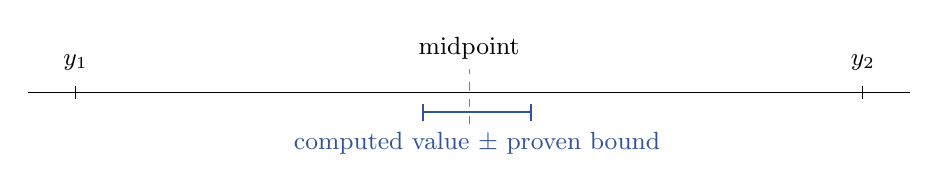
\begin{tikzpicture}[xscale=10]
    \draw (-0.06,0) -- (1.06,0);
    \draw (0,-0.08) -- (0,0.08) node[above=2pt, font=\small] {$y_1$};
    \draw (1,-0.08) -- (1,0.08) node[above=2pt, font=\small] {$y_2$};
    \draw[dashed, gray] (0.5,-0.4) -- (0.5,0.3)
    node[above, font=\small, black] {midpoint};
    \draw[thick, figblue, |-|] (0.44,-0.25) -- (0.58,-0.25);
    \node[below=3pt, font=\small, figblue] at (0.51,-0.28)
        {computed value $\pm$ proven bound};
        \end{tikzpicture}
        \caption{A hard case under round to nearest.  $y_1$ and $y_2$ are
        consecutive representable values. The proven error bound pins the
        exact result inside the marked interval, but the interval straddles the
        midpoint, so the rounding decision is unknown and a more precise path
        must run.}
        \label{fig:tmd}
        \Description{Visual aid for the concept described in the caption.}
    \end{figure}

    \subsection{Faithful rounding}

    Faithful rounding relaxes that requirement. The returned value may be either
    of the two floating-point neighbors around the exact result.

    Faithful rounding can be a useful interim target. It is not the same as
    correct rounding.

    \subsection{Ziv's strategy}

    Ziv's strategy uses a fast path and a
    fallback~\cite{ziv1991,muller,handbook}. Most inputs take the fast path.
    Rare hard cases take the accurate fallback. Correctly rounded libraries
    such as CRlibm use this pattern~\cite{crlibm}.

    \subsection{Hard cases}

    Hard cases turn up even in small samples. The script
    \path{docs/approximating_functions/sollya/hard_case_scan.sollya}
    walks a grid of 4097 doubles, evaluates \texttt{exp} of each to 300 bits,
    and measures the distance from each exact result to its nearest rounding
    boundary:

    \begin{lstlisting}[style=output]
samples: 4097
hardest input found: 0.4664154052734375
distance to rounding boundary in ulps: 8.2133230542e-5
extra bits needed to decide: 13.57
    \end{lstlisting}


    \begin{checkpoint}
        Mini exercise: decide whether the fast path is enough. Suppose the fast
        path returns an interval of possible exact results that lies wholly on one
        side of the rounding midpoint. Then suppose another input returns an
        interval that straddles the midpoint.
        \begin{enumerate}
            \item Which input can be rounded immediately?
            \item Which input needs the accurate fallback?
            \item Why is the second input called a hard case?
        \end{enumerate}
    \end{checkpoint}

    Four thousand ordinary inputs already contain one whose rounding decision
    needs the exact result to about 14~bits past the 53-bit format. Scale
    the sample up and the worst case keeps getting worse, roughly one extra
    bit per doubling. Exhaustive searches over the entire binary64 format,
    pioneered by Lef\`evre and Muller, find inputs for \texttt{exp} and its
    relatives that need the result to more than 100~bits in total before the
    decision is safe~\cite{lefevre}.

    That search result is what sizes the accurate path. A second phase
    that computes to 120~bits, with a proven bound, decides every known hard
    case for the functions whose searches are complete, which is how
    correctly rounded libraries pick their fallback
    precision~\cite{crlibm,muller}.

    For some functions and formats the search is still open, especially for
    binary128 and for two-argument functions like \texttt{pow}, where
    algorithms such as Stehlé-Lefèvre-Zimmermann (SLZ) push the frontier~\cite{muller,handbook}. When
    the worst case is unknown, a library can still be correct by iterating
    Ziv's strategy with growing precision, but it cannot promise a bound on
    the slowest call.

% -----------------------------------------------------------------------


    \section{Special cases}

    Special cases are part of the function.

    Do these before the polynomial path. The algebra used by the kernel usually
    assumes finite normalized inputs in a reduced interval. NaNs, infinities,
    zeros, subnormals, overflow thresholds, and exact identities do not all pass
    through that algebra safely.

    Handle NaNs, infinities, signed zeros, subnormals, exact results, overflow,
    underflow, invalid operations, and divide-by-zero behavior before the
    approximation path.

    Keep the polynomial kernel inside the range where its algebra is valid.

    For each function, write the special-case table before writing the
    polynomial. Here is what that table looks like for binary64 \texttt{exp}
    under round to nearest:

    \begin{table}[tbp]
        \centering
        \begin{tabular}{lll}
            \toprule
            Input                                   & Result       & Flags              \\
            \midrule
            quiet NaN                               & the same NaN & none               \\
            signaling NaN                           & a quiet NaN  & invalid            \\
            $+\infty$                               & $+\infty$    & none               \\
            $-\infty$                               & $+0$         & none               \\
            $\pm 0$                                 & 1, exactly   & none               \\
            $x$ above about $709.8$                 & $+\infty$    & overflow, inexact  \\
            $x$ between about $-745.2$ and $-708.4$ & a subnormal  & underflow, inexact \\
            $x$ below about $-745.2$                & $+0$         & underflow, inexact \\
            $|x|$ below about $2^{-54}$, nonzero    & 1            & inexact            \\
            \bottomrule
        \end{tabular}
    \end{table}

    Each threshold is a specific double that the implementation must get
    right, and the approximate values above are only signposts. The table
    also shifts with the rounding mode. Under \texttt{FE\_DOWNWARD} an
    overflowing \texttt{exp} must return the largest finite double rather
    than infinity, the tiny-input result moves off~1, and the underflow
    boundary moves. Keep one table per mode, or one table with a column per
    mode.

    \begin{figure}[tbp]
        \centering
        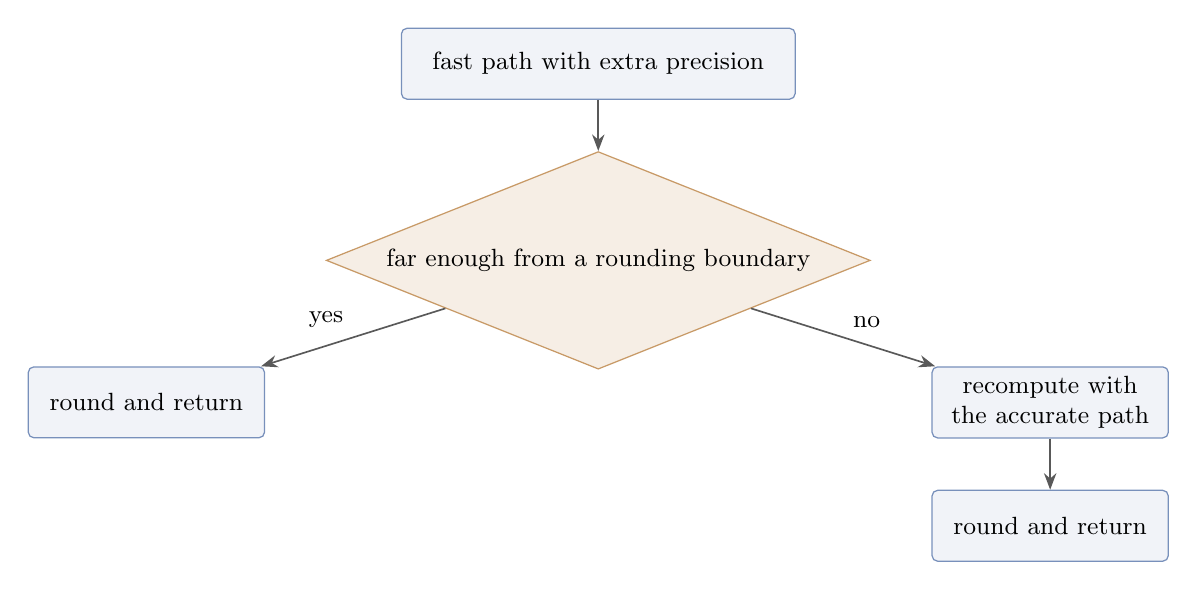
\begin{tikzpicture}[node distance=0.65cm and 2.5cm]
    \node (fast) [flowbox, minimum width=5cm] {fast path with extra precision};
    \node (dec)  [decisionbox, below=of fast] {far enough from a rounding boundary};
    \node (ret1) [flowbox, minimum width=3cm, below left=of dec]  {round and return};
    \node (acc)  [flowbox, minimum width=3cm, below right=of dec] {recompute with\\the accurate path};
    \node (ret2) [flowbox, minimum width=3cm, below=of acc]       {round and return};

    \draw[arrow] (fast) -- (dec);
    \draw[arrow] (dec) -- node[above left,  font=\small]{yes} (ret1);
    \draw[arrow] (dec) -- node[above right, font=\small]{no}  (acc);
    \draw[arrow] (acc) -- (ret2);
        \end{tikzpicture}
        \caption{Ziv's strategy as a fast-path test with a precise fallback.}
        \label{fig:ziv}
        \Description{Visual aid for the concept described in the caption.}
    \end{figure}

    Special cases are often where an implementation first reveals whether it was
    designed from the contract or from the ordinary finite path. The finite path
    is only one part of the function.


    \begin{checkpoint}
        Mini exercise: sort inputs before the kernel. For a new \texttt{log}
        implementation, classify these before any polynomial runs:
        \begin{enumerate}
            \item $x = 1$
            \item $x = +0$
            \item $x < 0$
            \item $x = +\infty$
            \item positive subnormal $x$
        \end{enumerate}
    \end{checkpoint}

% -----------------------------------------------------------------------


    \section{Rounding modes and dispatch policy}

    A library function should match the C++ math contract for the function being
    implemented. That includes finite values, special cases, overload behavior,
    return type, NaNs, infinities, signed zeros, subnormals, overflow, underflow,
    and rounding modes.

    For floating-point math functions, a strong target is correct behavior under
    all four IEEE rounding modes from Section~\ref{sec:roundingmodes}.

    That affects dispatch.

    A compiler builtin or platform libm call should not be assumed correct
    outside round-to-nearest. If a runtime path uses a builtin, SIMD
    implementation, or platform function that is only known safe under
    \texttt{FE\_TONEAREST}, the dispatcher must check the live rounding mode
    first.

    Directed modes should route to the generic kernel unless that fast path has
    been proved and tested for the active mode.

    The public header should not bypass that guard at runtime. Constant evaluation
    may use an eligible \texttt{constexpr} builtin when it satisfies the same
    edge-case and accuracy policy. Runtime calls should go through the runtime
    dispatcher so the live rounding mode is observed.

    That is part of the function contract. A polynomial that works under
    round-to-nearest is not automatically correct under \texttt{FE\_UPWARD},
    \texttt{FE\_DOWNWARD}, or \texttt{FE\_TOWARDZERO}. The final rounding step,
    signed-zero cases, overflow thresholds, and underflow behavior may depend on
    the active mode.

% -----------------------------------------------------------------------


    \section{Tool roles}

    Each tool answers a different question. Keeping those questions separate is
    what prevents a polynomial bound from being mistaken for a whole-function
    proof.

    \subsection{Sollya}

    Sollya bounds approximation error for a stated function, interval, error model,
    and coefficient format. That step does not cover reduction, evaluation,
    reconstruction, or final rounding.

    \subsection{Gappa}

    Gappa handles floating-point error bounds in straight-line
    code~\cite{gappapaper}.

    This fits Horner kernels, Estrin kernels, compensated sums, split constants,
    FMA sequences, and reconstruction fragments where the operation order is
    fixed.

    Sollya bounds the mathematical approximation error. Gappa helps bound the
    floating-point evaluation error. A worked account of certifying a real
    elementary function this way is given in~\cite{gappacert}.

    \subsection{Rocq}

    Rocq is an interactive theorem prover.

    Reach for it when the proof needs a larger machine-checked structure: definitions,
    lemmas, interval facts, rounding facts, and the link between local Gappa
    proofs and the function-level theorem.

    Rocq belongs to the high-assurance path, not the first pass for every
    function.

    \subsection{MPFR}

    MPFR is the independent oracle~\cite{mpfrpaper}.

    MPFR testing is not a proof, but it is the usual way to validate an
    implementation at scale. Test random inputs, boundary inputs, subnormals,
    overflow and underflow thresholds, exact cases, hard reduction cases, hard
    rounding cases, and every supported rounding mode.

    Measure ULP error. Do not rely on printed decimal comparisons. The
    harness from the sine example, with its order-preserving bit mapping, is
    the reusable core of such a suite.

    \subsection{SageMath}

    SageMath is useful for symbolic manipulation, series expansion, exact rational
    arithmetic, continued fractions, interval experiments, and prototype
    derivations.

    For example, before writing a \texttt{log1p} kernel, inspect:
    \[ \frac{\log(1+x)}{x} \]

    Before writing a trig reducer, inspect continued-fraction approximants of
    $\pi/2$.

    SageMath is a scratch tool. Sollya is the production coefficient path.

% -----------------------------------------------------------------------


    \section{Checklist for a new function}

    \subsection{Specify the target}

    Write down the function, supported formats, supported rounding modes, domain,
    special cases, accuracy target, and whether the goal is correct rounding,
    faithful rounding, or a stated ULP bound.

    Do this before writing coefficients or special-case code.

    \subsection{Choose the reduction}

    Decide how the input maps into a small interval.

    \begin{table}[tbp]
        \centering
        \begin{tabular}{ll}
            \toprule
            Function            & Typical reduction                                     \\
            \midrule
            $\exp(x)$           & $2^k$ times $\exp(r)$                                 \\
            $\log(x)$           & mantissa and exponent split                           \\
            trig                & reduction modulo $\pi/2$ or $\pi/4$                   \\
            $\mathrm{pow}(x,y)$ & special integer paths, logarithmic paths, exact cases \\
            \bottomrule
        \end{tabular}
    \end{table}

    Also decide how much precision the reduction carries.

    Record the sign, exponent, and significand split when the function uses it.

    \subsection{Define the kernel}

    Write the exact function that Sollya will approximate. Do not start with the
    public function name. Start with the expression that remains after reduction,
    table lookup, cancellation removal, or symmetry has done its work.

    This may be $\sin(r)$, $\sin(r)/r$, $\exp(r)$, $\mathrm{expm1}(r)/r$,
    $\log(1+r)/r$, a table residual, or another transformed function.

    \subsection{Choose the interval}

    Write the interval explicitly.
    \begin{align*}
        r &\in \left[-\frac{\ln 2}{2},\, \frac{\ln 2}{2}\right] \\[4pt]
        r &\in \left[-\frac{\pi}{4},\, \frac{\pi}{4}\right]
    \end{align*}

    An approximation proof only holds on the interval that was checked.

    \subsection{Choose the error model}

    Choose absolute error, relative error, or a weighted error.

    Prefer relative error when it matches ULP behavior. Switch to absolute error
    or a transformed kernel when relative error is ill-conditioned.

    \subsection{Generate coefficients}

    \texttt{guessdegree} gives a first degree estimate. Test nearby degrees.

    \texttt{fpminimax} is the production coefficient tool.

    \begin{lstlisting}[style=sollya]
prec = 200!;
display = hexadecimal!;
    \end{lstlisting}

    Generate coefficients in the same formats used by the implementation.

    \subsection{Generate the tables}

    For each lookup table, record the invariant.

    At minimum, write down the index formula, the represented real value, the
    split format, the exactness constraint, the residual interval, and the
    precision tier that consumes the table.

    Generate separate tables for separate precision tiers when the split or
    exactness constraint changes.

    For log-style tables, record the residual formula, such as
    $u = r_i(1 + m_x) - 1$, and the correction term supplied by the table.

    \subsection{Check the approximation}

    \texttt{dirtyinfnorm} is fine for quick iteration.  \texttt{supnorm} is the
    recorded bound.

    Record the interval, polynomial degree, coefficient formats, error model,
    and bound.

    \subsection{Choose the evaluation scheme}

    Choose Horner, Estrin, compensated Horner, double-word evaluation, or a
    hybrid.

    Treat the evaluation choice as part of the proof.

    \subsection{Choose the precision tiers}

    Decide which inputs use the fast path and which inputs need an accurate path.

    For float, double or double-double may be enough for many fast paths.

    For double, expect a double-double-like fast path and a wider accurate path
    for hard cases.

    Use dyadic formats when the accurate path needs fixed precision and wider
    exponent range.

    \subsection{Prove the evaluation error}

    Bound the floating-point error from the actual operation sequence.

    Run Gappa where possible. The approximation error alone is not enough.

    Keep the total error budget visible. The polynomial bound is only one term.

    \subsection{Reconstruct and round}

    Undo the reduction. Handle scaling, quadrant selection, sign reconstruction,
    table lookup, compensated addition, overflow, underflow, and double-rounding
    hazards where they apply.

    If the target is correct rounding, handle hard-to-round inputs or provide a
    bounded strategy that covers them.

    \subsection{Validate}

    Compare against MPFR over random, structured, boundary, subnormal, overflow,
    underflow, cancellation-heavy, and adversarial inputs.

    Run every supported rounding mode.

    \subsection{Record the status}

    Document supported formats, supported rounding modes, maximum observed ULP,
    proven bound if one exists, unsupported cases, known gaps, test coverage,
    oracle used, and the relevant Sollya, Gappa, SageMath, or Rocq artifacts.

% -----------------------------------------------------------------------


    \section{Where this lives in a library}

    Most implementations end up with the same pieces: special-case handling,
    reduction constants, approximation coefficients, an evaluation kernel,
    reconstruction logic, rounding-mode handling, oracle tests, and status notes.

    Generated constants are part of the algorithm. If the interval, coefficient
    format, polynomial degree, table split, or evaluation order changes, the
    proof needs review.

    Keep public APIs clean. Put function-specific machinery in internal support
    code. Keep kernels small enough to audit. Store or document enough
    information to regenerate the constants.

    If a function is only faithful, say so. If only round-to-nearest has been
    validated, say so. If directed modes are not covered, say so.

    Do not imply a stronger contract than the proof and tests support.

% -----------------------------------------------------------------------


    \section{Other approaches}

    \subsection{Traditional libm workflow}

    In practice, the workflow matches Figure~\ref{fig:ziv}, with explicit bounds
    on floating-point evaluation error before the final rounding argument. Sollya
    and Gappa fit this structure naturally.

    \subsection{RLIBM-style result approximation}

    RLIBM, a project name used for result-oriented libm generation, uses a different target~\cite{rlibm}.

    The traditional route approximates the real function, then proves that
    rounding gives the desired floating-point result.

    RLIBM generates polynomials that target the correctly rounded floating-point
    result directly. The polynomial is trying to land inside the interval of
    real values that round to the right floating-point answer.

    Not the default workflow in this guide. Worth studying for correctly
    rounded float functions, generated libraries, and multi-format work.

    \subsection{CRlibm and CORE-MATH}

    Correctly Rounded mathematical library (CRlibm) is useful for studying
    Ziv-test based correctly rounded functions~\cite{crlibm}.

    CORE-MATH is useful for modern correctly rounded elementary functions with
    compact implementations and proof-oriented notes~\cite{coremath}.

    Study the structure: reduction, approximation, reconstruction, hard cases,
    proof.

% -----------------------------------------------------------------------


    \section{Minimal Sollya template}

    Start from the script in Section~\ref{sec:sollyaexample}. For a
    reproducible production script,
    also print the certified bound and the coefficient forms:

    \begin{lstlisting}[style=sollya]
eps_cert = supnorm(p, f, I, relative, 1b-40);
print("certified relative error:", eps_cert);

print("certified relative error bits:", log2(eps_cert));

print("canonical:");
canonical(p);

print("horner:");
horner(p);
    \end{lstlisting}

    Keep the script with the implementation or proof tooling. Constants in
    source should be reproducible from the script.

% -----------------------------------------------------------------------


    \section{Minimal SageMath scratch template}

    Use SageMath before the production Sollya script when the algebra is still
    being explored.

    \begin{lstlisting}[style=shell]
var('x')

f = log(1 + x) / x
series(f, x, 0, 10)
    \end{lstlisting}

    For continued fractions:
    \begin{lstlisting}[style=shell]
continued_fraction(pi / 2).convergents()[:10]
    \end{lstlisting}

    For exact rational checks:
    \begin{lstlisting}[style=shell]
R = RationalField()
a = R(355) / R(113)
a - pi.n(100)
    \end{lstlisting}

    Treat these as exploration unless the exact claim is recorded and checked as
    part of the proof.

% -----------------------------------------------------------------------


    \section{Measuring performance}

    Speed numbers are as easy to get wrong as accuracy numbers, and wrong in
    quieter ways.

    Benchmark the function the way applications call it. Feed inputs from a
    prefilled array rather than a constant, so the compiler cannot fold the
    call away and the branch predictor cannot memorize one special-case
    path. Consume every result, a summed sink variable is enough. Measure
    latency and throughput separately and label which is which: latency
    chains each call's result into the next call's input, while throughput
    runs independent calls. On kernels that vectorize well the two can
    differ by several times.

    Input distribution is part of the result. A benchmark of
    \texttt{exp} over $[0, 1]$ never visits the subnormal, overflow, or
    accurate-path branches, and a benchmark of \texttt{sin} over
    $[10^{15}, 10^{16}]$ does nothing but large-argument reduction. Report
    the range with every number, and benchmark the slow paths separately so
    a regression in them is visible at all.

    Compare against the platform libm compiled with the same flags, on the
    same input set, in the same harness. Numbers taken from different
    harnesses are not comparable. Once the algorithm is fixed,
    instruction-level profilers and hardware counters help with the last
    factors, but the biggest levers are design choices: polynomial degree,
    table size against cache pressure, and how rarely the accurate path
    triggers.

% -----------------------------------------------------------------------


    \section{Citation policy}

    Citations use ACM numeric style with \texttt{ACM-Reference-Format.bst}.
    Prefer full author names and stable DOI or URL fields in the bibliography.

    \begin{table}[tbp]
        \centering
        \begin{tabular}{>{\raggedright\arraybackslash}p{5.3cm}>{\raggedright\arraybackslash}p{6.1cm}}
            \toprule
            Source & Typical use in this guide                                        \\
            \midrule
            IEEE 754-2019~\cite{ieee}
            & Required operations, rounding modes, exceptions, NaNs, infinities,
            signed zeros, subnormals \\
            Muller, \emph{Elementary Functions}~\cite{muller}
            & Minimax approximation, Remez, range reduction, Cody-Waite,
            Payne-Hanek, Ziv tests \\
            \emph{Handbook of Floating-Point Arithmetic}~\cite{handbook}
            & ULPs, FMA, double-word arithmetic, compiler hazards, Gappa, MPFR \\
            Sollya~\cite{sollya}
            & Command syntax and coefficient generation                        \\
            Gappa~\cite{gappa}
            & Straight-line floating-point error proofs                        \\
            de~Dinechin, Lauter, Muller~\cite{dinechinlog}
            & Production table-based log with correct-rounding proof           \\
            de~Dinechin, Lauter, Melquiond~\cite{gappacert}
            & Certifying an elementary function with Gappa                     \\
            Ziv~\cite{ziv1991}, Payne and Hanek~\cite{payne1983},
            Lef\`evre and Muller~\cite{lefevre}
            & Original papers for the named algorithms and worst-case searches \\
            Brisebarre and Chevillard~\cite{brisebarre2007}
            & The method behind \texttt{fpminimax}                             \\
            Tool papers~\cite{sollyapaper,mpfrpaper,gappapaper}
            & Citable descriptions of Sollya, MPFR, and Gappa                  \\
            Rocq~\cite{rocq}
            & Machine-checked proof structure                                  \\
            SageMath~\cite{sagemath}
            & Symbolic exploration before production scripts                   \\
            MPFR~\cite{mpfr}
            & Oracle reference behavior                                        \\
            RLIBM~\cite{rlibm}
            & Direct approximation of the correctly rounded result             \\
            Goldberg~\cite{goldberg}, Oracle Numerical Computation Guide (NCG)~\cite{oracle}
            & Introductory floating-point background                           \\
            \bottomrule
        \end{tabular}
    \end{table}

% -----------------------------------------------------------------------


    \section{Further reading}

    The bibliography lists the works cited in the body. The notes below give a
    reading path instead: free resources first, then paid books for deeper
    derivations. Each entry lists a URL and what it covers. Where an entry has a
    citable paper behind it, the bibliography entry is the stable reference.

    \subsection{Free resources}

    \subsubsection{First pass on floating point.}

    \emph{Oracle reprint of Goldberg, What Every Computer Scientist Should Know
    About Floating-Point Arithmetic.}
    \url{https://docs.oracle.com/cd/E19957-01/806-3568/ncg_goldberg.html}\\
    Introductory floating-point article. Covers rounding, guard digits,
    cancellation, ULPs, and IEEE arithmetic.

    \emph{The Floating-Point Guide.}
    \url{https://floating-point-gui.de/}\\
    Short beginner reference on binary floating-point behavior, not libm design.

    \emph{IEEE~754-2019 official page.}
    \url{https://standards.ieee.org/standard/754-2019.html}\\
    Official standard page. The full text is not free on every access path.

    \subsubsection{Sollya and approximation work.}

    \emph{Sollya official site.}
    \url{https://www.sollya.org/}\\
    Tool site and current manual. Minimax approximation, constrained
    coefficients, and certified supremum-norm checks.

    \emph{Sollya} \texttt{fpminimax} documentation.
    \url{https://www.sollya.org/sollya-current/help.php?name=fpminimax}\\
    Command reference for production coefficients in requested floating-point
    formats.

    \emph{Sollya} \texttt{supnorm} documentation.
    \url{https://www.sollya.org/sollya-current/help.php?name=supnorm}\\
    Recorded approximation bounds. Run after quick \texttt{dirtyinfnorm} checks.

    \subsubsection{Proof and validation tools.}

    \emph{Gappa user guide.}
    \url{https://gappa.gitlabpages.inria.fr/gappa/index.html}\\
    Straight-line floating-point and fixed-point error proofs after Sollya.

    \emph{Rocq Prover reference manual.}
    \url{https://rocq-prover.org/refman}\\
    Machine-checked proof structure beyond local Gappa bounds.

    \emph{GNU Multiple Precision Floating-Point Reliable Library (MPFR) official site.}
    \url{https://www.mpfr.org/}\\
    High-precision oracle with correct rounding.

    \emph{SageMath documentation.}
    \url{https://doc.sagemath.org/}\\
    Symbolic exploration before production Sollya scripts: series, exact
    rationals, and continued fractions.

    \subsubsection{Implementations and current research.}

    \emph{LLVM libc math status.}
    \url{https://libc.llvm.org/math/}\\
    LLVM libc math accuracy table, including functions marked correctly rounded
    in all four rounding modes.

    \emph{CORE-MATH project.}
    \url{https://core-math.gitlabpages.inria.fr/}\\
    Compact correctly rounded implementations and proof-oriented notes.

    \emph{CORE-MATH paper.}
    \url{https://inria.hal.science/hal-03721525v3/file/core-math-final.pdf}\\
    Project goals and design direction.

    \emph{RLIBM project page.}
    \url{https://people.cs.rutgers.edu/~sn349/rlibm/}\\
    Polynomials that target the correctly rounded floating-point result directly.

    \emph{RLIBM-ALL paper.}
    \url{https://arxiv.org/abs/2108.06756}\\
    Multi-format, multi-rounding-mode RLIBM.

    \emph{RLIBM-MultiRound paper.}
    \url{https://arxiv.org/abs/2504.07409}\\
    Rounding-mode switching cost and methods that avoid depending on the live
    mode.

    \emph{CRlibm report.}
    \url{https://ens-lyon.hal.science/ensl-01529804v1/document}\\
    Correctly rounded elementary functions and Ziv-style design.

    \emph{Fast and correctly rounded logarithms in double-precision.}
    \url{https://ens-lyon.hal.science/ensl-00000007v2}\\
    Production-grade version of the table-based log core built in
    Section~\ref{sec:log2}, with the full proof structure~\cite{dinechinlog}.

    \emph{Certifying the floating-point implementation of an elementary
    function using Gappa.}
    \url{https://arxiv.org/abs/0801.0523}\\
    End-to-end account of proving a real kernel's evaluation
    error~\cite{gappacert}.

    \emph{SIGPLAN blog introduction to RLIBM.}
    \url{https://blog.sigplan.org/2021/08/26/high-performance-correctly-rounded-math-libraries-for-32-bit-floating-point-representations/}\\
    Readable introduction to the RLIBM approach without the paper
    formalism~\cite{rlibmblog}.

    \subsubsection{Performance-oriented implementation references.}

    \emph{SLEEF paper.}
    \url{https://www.shibatch.net/sleef/}\\
    Portable vectorized elementary functions with explicit vector paths and
    accuracy targets~\cite{sleef}.

    \emph{LLVM libc math slides.}
    \url{https://libc.llvm.org/math/}\\
    Modern CPU instructions, FMA, and rounding instructions in LLVM libc math
    work.

    \emph{Arm Optimized Routines.}
    \url{https://www.arm.com/why-arm/technologies/compute-library}\\
    Target-specific scalar and vector math routines for Arm CPUs~\cite{arm}.

    \emph{Agner Fog optimization manuals.}
    \url{https://www.agner.org/optimize/}\\
    CPU microarchitecture, instruction timing, and low-level performance
    notes~\cite{fog}.

    \emph{Intel optimization manual.}
    \url{https://www.intel.com/content/www/us/en/developer/articles/technical/intel-sdm.html}\\
    Intel x86 tuning and instruction behavior~\cite{intel}.

    \emph{AMD Zen optimization guide.}
    \url{https://developer.amd.com/resources/developer-guides-manuals/}\\
    AMD-specific tuning for Zen-family processors~\cite{amd}.

    \subsubsection{Survey and background papers.}

    \emph{Floating-point arithmetic, Acta Numerica survey.}
    \url{https://www.cambridge.org/core/journals/acta-numerica/article/floating-point-arithmetic/287C4D5F6D4A43FBEEB1ABED2A405AAF}\\
    Modern survey of floating-point arithmetic and IEEE behavior.

    \emph{Gappa paper, Certification of bounds on expressions involving rounded
    operators.}
    \url{https://arxiv.org/abs/cs/0701186}\\
    Paper behind the Gappa tool.

    \emph{MPFR paper, A Multiple-Precision Binary Floating-Point Library with
    Correct Rounding.}
    \url{https://inria.hal.science/inria-00070266v1/document}\\
    Design of the usual high-precision oracle.

    \subsection{Paid books and standards}

    \subsubsection{Best main book for elementary functions.}

    \emph{Elementary Functions: Algorithms and Implementation}, Jean-Michel
    Muller, Springer.
    \url{https://link.springer.com/book/10.1007/978-1-4899-7983-4}\\
    Exp, log, trig functions, range reduction, polynomial approximation, table
    methods, and correct rounding.

    \subsubsection{Best main book for floating-point arithmetic.}

    \emph{Handbook of Floating-Point Arithmetic}, 2nd edition, Springer.
    \url{https://link.springer.com/book/10.1007/978-3-319-76526-6}\\
    Floating-point formats, rounding, ULPs, FMA, exceptions, compiler issues,
    Gappa, MPFR, and formal verification.

    \subsubsection{Strong general book on finite precision error.}

    \emph{Accuracy and Stability of Numerical Algorithms}, Nicholas J. Higham,
    SIAM.
    \url{https://epubs.siam.org/doi/10.1137/1.9780898718027}\\
    Numerical error, stability, and finite precision analysis, not libm design.

    \subsubsection{Shorter IEEE floating-point book.}

    \emph{Numerical Computing with IEEE Floating Point Arithmetic}, Michael L.
    Overton, SIAM.
    \url{https://epubs.siam.org/doi/book/10.1137/1.9780898718072}\\
    Shorter IEEE floating-point introduction than the Handbook.

    \subsubsection{Historical libm implementation reference.}

    \emph{Software Manual for the Elementary Functions}, Cody and Waite.
    \url{https://www.amazon.com/Elementary-Functions-Prentice-Hall-computational-mathematics/dp/0138220646}\\
    Classic libm structure: reduction, rational approximation, special cases, and
    implementation constants. Not a modern correctness target.

    \subsubsection{Official floating-point standard.}

    \emph{IEEE 754-2019 official standard page.}
    \url{https://standards.ieee.org/standard/754-2019.html}\\
    Authoritative standard for floating-point formats, rounding attributes,
    exceptions, NaNs, infinities, signed zeros, subnormals, and required
    operations.

% -----------------------------------------------------------------------
    \appendix


    \section{Checkpoint answers}

    These answers are collected here so the checkpoint boxes can be used as
    exercises while reading.

    \subsection*{Small sine kernel}

    \begin{enumerate}
        \item The quotient $\sin(x)/x$ is smooth and close to~1 near zero, so its
        relative error stays well behaved. Working in $z = x^2$ also uses the odd
        symmetry of sine, which cuts the number of polynomial terms.
        \item The Sollya bound and the tests hold only on the stated interval, so
        both must be rerun. The degree may also need to grow, because the old
        polynomial was only certified on $[-1/16, 1/16]$.
        \item Hexadecimal literals store exactly the bits Sollya printed. A
        decimal spelling can introduce another rounding step before the compiler
        stores the coefficient.
    \end{enumerate}

    \subsection*{Small log2 core}

    \begin{enumerate}
        \item The reciprocal table shrinks the interval the polynomial must cover.
        A smaller residual interval usually lowers the degree, tightens the error
        bound, or both.
        \item The high part is rounded to fewer bits so that adding it to the
        exponent term is easier to prove exact for the intended path. The low part
        carries the leftover correction through the compensated tail.
        \item The residual $u$ lives in a small interval around zero, where a
        low-degree polynomial is accurate. Dividing by $u$ removes the zero of
        $\log_2(1 + u)$, so the relative-error problem stays well behaved.
    \end{enumerate}

    \subsection*{Cody-Waite reduction drift}

    $k = 1443$, the residual is $r \approx -0.2114$, and the drift is
    $1443 \cdot 9.4 \cdot 10^{-18} \approx 1.36 \cdot 10^{-14}$, which is
    about 490~ULPs of $r$. The input grew 33~times over the $x = 30$ case and
    the drift grew with it, because the drift scales with $k$. That scaling is
    why the split is not optional.

    \subsection*{ULP scale from absolute error}

    Near magnitude~1, binary64 ULP size is $2^{-52}$, so an absolute error of
    $2^{-55}$ is $2^{-3}$ ULP, or one eighth of an ULP. Near magnitude $2^{-10}$,
    ULP size is $2^{-62}$, so the same absolute error is $2^7 = 128$ ULPs. That is
    why a flat absolute-error target can be misleading when the result spans many
    binades.

    \subsection*{Spending the Sollya bit budget}

    A $2^{-57.8}$ relative approximation bound gives about 57.8 bits before the
    other stages spend any margin. Binary64 round-to-nearest needs about 53 bits
    for a simple half-ULP argument, so spending 5 bits leaves about $57.8 - 5 =
    52.8$ bits. That is already tight or slightly over budget, depending on how
    conservative the bound is. The fix is not wishful rounding; it is a better
    polynomial, a smaller interval, a more accurate evaluation path, or a fallback.

    \subsection*{Normalizing $0.15625$}

    $0.15625 = 5/32 = 1.25 \cdot 2^{-3}$, so $m = 1.25$ and $e = -3$.
    Therefore:
    \[
        \log_2(0.15625) = -3 + \log_2(1.25).
    \]
    The exponent part is exact. The table and polynomial only need to handle
    $\log_2(1.25)$ on the fixed interval $[1,2)$.

    \subsection*{Walking one log table row}

    For $m = 1.40$ and $B = 16$, the index is
    $i = \lfloor (1.40 - 1)16 \rfloor = \lfloor 6.4 \rfloor = 6$. The bucket
    center is $c_6 = 1 + (6 + 1/2)/16 = 1.40625$. Using $r_6 \approx 1/c_6$ gives
    $u \approx 1.40/1.40625 - 1 \approx -0.00444$. The residual is small and
    negative, which is exactly what the table is supposed to achieve.

    \subsection*{Choosing Horner or Estrin}

    Estrin has the shorter dependency chain because independent groups can be
    evaluated in parallel. Horner is simpler to audit and prove because the source
    code, generated expression, and Gappa model can follow one linear chain of
    multiply-adds. On a target with slow FMA but good instruction-level
    parallelism, benchmark Estrin first, but keep the proof tied to the exact
    operation sequence that ships.

    \subsection*{Routing \texttt{pow} calls}

    $\mathrm{pow}(2,10)$ can use an integer-exponent or exact power-of-two path.
    $\mathrm{pow}(-2,3)$ needs the integer-exponent path and returns a negative
    result. $\mathrm{pow}(-2,0.5)$ is a special-case/domain error: finite negative
    base with non-integer exponent returns NaN. $\mathrm{pow}(1,\mathrm{NaN})$
    returns 1 by the special-case rules.

    \subsection*{Fast path or accurate fallback}

    If the proven interval lies wholly on one side of the rounding midpoint, the
    fast path can round immediately because every value in the interval chooses
    the same floating-point neighbor. If the interval straddles the midpoint, the
    fast path cannot decide. That input is a hard case because the exact result is
    too close to a rounding boundary for the current precision to prove the final
    bit.

    \subsection*{Sorting \texttt{log} inputs}

    $\log(1)$ is an exact special case returning $+0$. $\log(+0)$ returns
    $-\infty$ and raises divide-by-zero. A negative finite input returns NaN and
    raises invalid. $\log(+\infty)$ returns $+\infty$. A positive subnormal is a
    finite positive input, but it must be normalized before entering the ordinary
    reduced kernel.


    \section{Useful vocabulary}

    \begin{table}[H]
        \centering
        \begin{tabular}{p{3.8cm}p{8.5cm}}
            \toprule
            Term & Meaning                                                           \\
            \midrule
            argument reduction
            & A mapping from the public input to a smaller interval where
            approximation is easier. \\
            kernel
            & The exact function that is actually approximated after reduction. \\
            transformed kernel
            & A kernel rewritten to remove a zero, cancellation point, or unstable
            relative error. \\
            reduced interval
            & The interval on which the approximation bound is claimed.         \\
            residual
            & The small quantity that remains after a table lookup or other
            reduction step. \\
            reconstruction
            & The step that combines the reduced result with exponents, table
            constants, signs, or quadrants. \\
            minimax polynomial
            & A polynomial that minimizes the worst error on a stated interval. \\
            coefficient format
            & The floating-point or fixed-width format in which the implementation
            stores the coefficients. \\
            evaluation scheme
            & The operation order used to evaluate the polynomial, such as Horner
            or Estrin. \\
            table invariant
            & The exact real relation that a table entry is meant to support.   \\
            exactness constraint
            & A requirement that one later operation be exact or tightly bounded
            because of how a constant was split. \\
            faithful rounding
            & Returning one of the two floating-point neighbors of the exact
            result. \\
            correct rounding
            & Returning the value selected by the active rounding mode from the
            exact real result. \\
            hard case
            & An input whose exact result lies unusually close to a rounding
            boundary. \\
            oracle
            & An independent high-precision reference used for validation, usually
            MPFR in this workflow. \\
            fast path
            & The cheap path intended for ordinary inputs.                      \\
            accurate path
            & The slower path used when the fast path cannot justify the final
            rounding decision. \\
            binade
            & The interval between two consecutive powers of two. Floating-point
            spacing is constant inside one binade and changes at binade boundaries. \\
            unit in the last place (ULP)
            & The gap between consecutive floating-point values at a given
            magnitude. \\
            \bottomrule
        \end{tabular}
    \end{table}

% -----------------------------------------------------------------------


    \section{How the proof pieces fit together}

    Keep these obligations separate when reading or writing a proof note.

    \begin{enumerate}
        \item \textbf{Reduction bound:} distance between the computed reduced
        argument and the exact reduced argument.
        \item \textbf{Approximation bound:} distance between the mathematical
        polynomial and the kernel on the reduced interval.
        \item \textbf{Evaluation bound:} rounding error from the compiled operation
        sequence that evaluates the polynomial.
        \item \textbf{Reconstruction bound:} effect of split constants, exponent
        additions, sign fixes, and table lookups.
        \item \textbf{Rounding argument:} margin to a rounding boundary, or the need
        for a fallback path.
        \item \textbf{Oracle validation:} agreement with an independent reference
        over many inputs. Engineering evidence, not a proof certificate.
    \end{enumerate}

    Small approximation error does not fix bad reduction. A split table does
    not prove the polynomial. MPFR agreement does not certify the floating-point
    circuit. State which obligation each artifact covers.

    \clearpage
    \bibliographystyle{ACM-Reference-Format}
    \bibliography{approx_functions}

\end{document}
